% !TeX encoding = UTF-8
% !TeX program = xelatex
% !TeX spellcheck = en_US

\documentclass[degree=master]{thuthesis}
  % 学位 degree:
  %   doctor | master | bachelor | postdoc
  % 学位类型 degree-type:
  %   academic(默认)| professional
  % 语言 language
  %   chinese(默认)| english
  % 字体库 fontset
  %   windows | mac | fandol | ubuntu
  % 建议终版使用 Windows 平台的字体编译


% 论文基本配置,加载宏包等全局配置
% !TeX root = ./thuthesis-example.tex

% 论文基本信息配置

\thusetup{
  %******************************
  % 注意:
  %   1. 配置里面不要出现空行
  %   2. 不需要的配置信息可以删除
  %   3. 建议先阅读文档中所有关于选项的说明
  %******************************
  %
  % 输出格式
  %   选择打印版(print)或用于提交的电子版(electronic),前者会插入空白页以便直接双面打印
  %
  output = print,
  %
  % 标题
  %   可使用“\\”命令手动控制换行
  %
  title  = {鲁棒控制障碍函数的验证与综合:多级多项式优化和半定松弛},
  title* = {Verification and Synthesis of Robust Control Barrier Function: Multilevel Polynomial Optimization and Semidefinite Relaxation},
  %
  % 学位
  %   1. 学术型
  %      - 中文
  %        需注明所属的学科门类,例如:
  %        哲学、经济学、法学、教育学、文学、历史学、理学、工学、农学、医学、
  %        军事学、管理学、艺术学
  %      - 英文
  %        博士:Doctor of Philosophy
  %        硕士:
  %          哲学、文学、历史学、法学、教育学、艺术学门类,公共管理学科
  %          填写“Master of Arts“,其它填写“Master of Science”
  %   2. 专业型
  %      直接填写专业学位的名称,例如:
  %      教育博士、工程硕士等
  %      Doctor of Education, Master of Engineering
  %   3. 本科生不需要填写
  %
  % degree-name  = {工学学士},
  % degree-name* = {Bachelor of Engineering},
  %
  % 培养单位
  %   填写所属院系的全名
  %
  department = {电子工程系},
  %
  % 学科
  %   1. 学术型学位
  %      获得一级学科授权的学科填写一级学科名称,其他填写二级学科名称
  %   2. 工程硕士
  %      工程领域名称
  %   3. 其他专业型学位
  %      不填写此项
  %   4. 本科生填写专业名称,第二学位论文需标注“(第二学位)”
  %
  discipline  = {电子信息科学与技术},
  discipline* = {Electronic Information Science and Technology},
  %
  % 姓名
  %
  author  = {康书诚},
  author* = {Kang Shucheng},
  %
  % 指导教师
  %   中文姓名和职称之间以英文逗号“,”分开,下同
  %
  supervisor  = {张旭东, 教授},
  supervisor* = {Professor Zhang Xudong},
  %
  % 副指导教师
  %
  % associate-supervisor  = {陈文光, 教授},
  % associate-supervisor* = {Professor Chen Wenguang},
  %
  % 联合指导教师
  %
  % co-supervisor  = {某某某, 教授},
  % co-supervisor* = {Professor Mou Moumou},
  %
  % 日期
  %   使用 ISO 格式;默认为当前时间
  %
  % date = {2019-07-07},
  %
  % 是否在中文封面后的空白页生成书脊(默认 false)
  %
  include-spine = false,
  %
  % 密级和年限
  %   秘密, 机密, 绝密
  %
  % secret-level = {秘密},
  % secret-year  = {10},
  %
  % 博士后专有部分
  %
  % clc                = {分类号},
  % udc                = {UDC},
  % id                 = {编号},
  % discipline-level-1 = {计算机科学与技术},  % 流动站(一级学科)名称
  % discipline-level-2 = {系统结构},          % 专业(二级学科)名称
  % start-date         = {2011-07-01},        % 研究工作起始时间
}

% 载入所需的宏包

% 定理类环境宏包
\usepackage{amsthm}
% 也可以使用 ntheorem
% \usepackage[amsmath,thmmarks,hyperref]{ntheorem}

\thusetup{
  %
  % 数学字体
  % math-style = GB,  % GB | ISO | TeX
  math-font  = xits,  % stix | xits | libertinus
}

% 可以使用 nomencl 生成符号和缩略语说明
% \usepackage{nomencl}
% \makenomenclature

% 表格加脚注
\usepackage{threeparttable}

% 表格中支持跨行
\usepackage{multirow}

% 固定宽度的表格。
% \usepackage{tabularx}

% 跨页表格
\usepackage{longtable}

% 算法
\usepackage{algorithm}
\usepackage{algorithmic}

% 量和单位
\usepackage{siunitx}

% 参考文献使用 BibTeX + natbib 宏包
% 顺序编码制
\usepackage[sort]{natbib}
\bibliographystyle{thuthesis-numeric}

% 著者-出版年制
% \usepackage{natbib}
% \bibliographystyle{thuthesis-author-year}

% 本科生参考文献的著录格式
% \usepackage[sort]{natbib}
% \bibliographystyle{thuthesis-bachelor}

% 参考文献使用 BibLaTeX 宏包
% \usepackage[style=thuthesis-numeric]{biblatex}
% \usepackage[style=thuthesis-author-year]{biblatex}
% \usepackage[style=apa]{biblatex}
% \usepackage[style=mla-new]{biblatex}
% 声明 BibLaTeX 的数据库
% \addbibresource{ref/refs.bib}

% 定义所有的图片文件在 figures 子目录下
\graphicspath{{figures/}}

% 数学命令
\makeatletter
\newcommand\dif{%  % 微分符号
  \mathop{}\!%
  \ifthu@math@style@TeX
    d%
  \else
    \mathrm{d}%
  \fi
}
\makeatother

% hyperref 宏包在最后调用
\usepackage{hyperref}



\begin{document}

% 封面
\maketitle

% 学位论文指导小组、公开评阅人和答辩委员会名单
% 本科生不需要
% \input{data/committee}

% 使用授权的说明
\copyrightpage
% 将签字扫描后授权文件 scan-copyright.pdf 替换原始页面
% \copyrightpage[file=scan-copyright.pdf]

\frontmatter
% !TeX root = ../thuthesis-example.tex

% 中英文摘要和关键字

\begin{abstract}
  本文研究了具备加性不确定性和凸控制输入边界的仿射多项式系统中,鲁棒控制障碍函数的验证和综合问题。在上述系统条件下,控制障碍函数的验证和综合问题可表示为多级多项式优化问题。其中,验证问题包含三个级别的优化:系统不确定性、控制输入和系统状态;而综合问题对控制障碍函数的候选参数也进行了优化。研究表明,通过对系统不确定性和控制输入这两个优化级别使用KKT条件,验证问题可以简化为单级多项式优化问题,综合问题可以简化为最小-最大多项式优化问题。进一步地,我们可以使用多级半正定松弛求解上述两个问题:对于验证问题转化而来的单级多项式优化问题,我们应用Lasserre's Hierarchy这一矩松弛方法;对于综合问题转化来的最小-最大多项式优化问题,我们使用平方和优化方法获得优化问题未知值函数的不断紧逼的多项式下界,并再次调用Lasserre's Hierarchy以最大化下界。两种松弛方法都拥有渐进收敛到全局最优的理论保证。实验方面,我们对受控Van der Pol振荡器进行了深入研究,并对系统具备和不具备加性不确定性这两种情况分别进行了讨论。

  % 关键词用“英文逗号”分隔,输出时会自动处理为正确的分隔符
  \thusetup{
    keywords = {控制障碍函数,多项式优化,半定松弛,最小-最大优化},
  }
\end{abstract}

\begin{abstract*}
  In this paper, we study the verification and synthesis of robust control barrier functions for affine polynomial systems with additive uncertainty and convex control input bounds. Under the above system conditions, the verification and synthesis problem of the control barrier function can be expressed as multilevel polynomial optimization problems. Among them, the verification problem contains three levels of optimization: system uncertainty, control input, and system state; while the synthesis problem also optimizes the candidate parameters of the control barrier function. It is shown that by using KKT conditions for the two optimization levels of system uncertainty and control input, the verification problem can be reduced to a single-level polynomial optimization problem, and the synthesis problem can be reduced to a min-max polynomial optimization problem. Furthermore, we can use multi-level positive semi-definite relaxation to solve the above two problems: for the single-level polynomial optimization problem transformed from the verification problem, we apply the Lasserre's Hierarchy moment relaxation method; for the min-max polynomial problem transformed from the synthesis problem, we use the sum-of-squares optimization method to obtain an ever-tightening polynomial lower bound for the unknown value function of the optimization problem, and call Lasserre's Hierarchy again to maximize the lower bound. Both relaxation methods have theoretical guarantees of asymptotic convergence to the global optimum. In terms of experiments, we have conducted an in-depth study on the controlled Van der Pol oscillator, and discussed the two cases of the system with and without additive uncertainty.

  % Use comma as separator when inputting
  \thusetup{
    keywords* = {control barrier function, polynomial optimization, semidefinite relaxation, min-max optimization},
  }
\end{abstract*}


% 目录
\tableofcontents

% 插图和附表清单
% 本科生的插图索引和表格索引需要移至正文之后、参考文献前
% \listoffiguresandtables  % 插图和附表清单(仅限研究生)
% \listoffigures           % 插图清单
% \listoftables            % 附表清单

% 符号对照表
% \input{data/denotation}


% 正文部分
\mainmatter
% !TeX root = ../thuthesis-example.tex

\chapter{引言}

\section{鲁棒控制障碍函数简介}
安全性在智能与自动系统中至关重要。在控制领域中,基于能量函数的安全控制算法被广泛使用。这一类算法将系统状态约束在某一“安全集合”中。其中,控制障碍函数\cite{ames2014cdc-cbforigin} 引起了越来越多的研究兴趣。控制障碍函数将安全集编码为其控制不变的零上水平集:亦即,如果系统在安全集中启动,则始终存在一控制输入序列,将系统状态保持在这一安全集合中。于此同时,由于动态不确定性在现实世界的应用中无处不在,针对系统不确定性的鲁棒控制障碍函数随之出现,以确保系统在存在不确定性的情况下保持安全。

\section{鲁棒控制障碍函数的验证和综合问题}
在涉及(鲁棒)控制障碍函数的现有文献中,大家将注意力主要集中在CBF的部署问题上:假设已经获得了一个控制障碍函数,在此基础上通过二次规划方法\cite{taylor2020acc-robustqp}或者二阶锥规划\cite{buch21csl-robust}生成一个安全控制器。然而,仍有两个挑战未被解决:如何去验证与综合一个鲁棒安全控制函数?
\begin{enumerate}
    \item 验证问题。若现在给定一个候选鲁棒控制障碍函数,对于其上水平集中包含的所有系统状态以及所有可能的动力学不确定性,我们需要验证是否总是存在一个合法的控制输入,使得系统状态能维持在这一上水平集内。
    \item 综合问题。在一个函数空间中,寻找一个合法的鲁棒控制障碍函数(并且验证它的正确性)。
\end{enumerate}

针对多项式动力学系统以及简单的多面体控制输入边界,现有的工作将综合问题转化为一凸的平方和优化问题~\cite{clark22arxiv-cbf,dai2022arxiv-clfcbfsynveri},并将综合问题转化为一个非凸的双线性平方和优化问题~\cite{wang2018acc-permissive,zhao22arxiv-cbfsos}。在上述方法中,存在两个缺陷。第一,双线性平方和优化算法通过交替下降方法进行优化求解,而该方法无法提供全局收敛性的理论保证。第二,此类方法无法处理动力学模型中的不确定性以及更为广泛的(凸)控制输入约束。

\section{主要贡献}
本文针对的仿射多项式动力学系统具有如下特性:(1)系统模型中的动力学不确定性为有界、加性且与系统状态有关的。(2)系统的控制信号输入被约束在任意的凸包中。在上述模型之上,我们研究鲁棒控制障碍函数的验证和综合问题。首先,我们将上述两个问题进行了符号语言上的统一与公式化:它们均可以被表示为多级多项式优化问题{\color{red} AAA}~\cite{bennett22mp-hierarchical}。特别地,对于一个参数化的鲁棒控制障碍函数候选,验证问题被转化为三级多项式优化问题:我们由外向内,分别优化不确定性,控制信号输入,以及系统状态。综合问题则转换为了一个四级的多项式优化问题,附带额外搜索最佳参数{\color{red} AAA}。尽管多级优化问题难以处理,但本文研究表明,在凸控制约束和有界不确定性这两大前提下,我们可以通过KKT最优性条件以解析解的形式消除内部两级优化(不确定性和控制)。因此,验证问题可以减少到状态上的单级多项式优化问题,综合问题则可以减少到状态和参数上的最小-最大多项式优化问题{\color{red} AAA}。在完成问题表征后,我们采用多级半正定规划松弛来近似求解多项式优化问题,并指出该系列数学处理方法具有全局收敛性保证{\color{red} AAA}。更为具体地,针对由验证问题转化而来的单级多项式优化问题,我们采用Lasserre's Hierarchy这一矩松弛方法~\cite{lasserre01siopt-global}。对于最小-最大多项式优化问题,我们采用双阶段松弛方法{\color{red} AAA}~\cite{lasserre11jgo-minmaxpop}:在第一阶段,我们使用平方和优化方法获得优化问题未知值函数的不断紧逼的多项式下界;在第二阶段,我们再一次通过Lasserre's Hierarchy最大化多项式下界,来搜索鲁棒控制障碍函数的有效参数。读者可以参看图{\color{red} CCC}以直观地感受我们的方法:图中,蓝色虚线是未知值函数,实线是通过平方和优化方法找到的多项式下界。我们对受控Van der Pol振荡器进行了深入研究,并对系统具备和不具备加性不确定性这两种情况分别进行了讨论{\color{red} AAA}。

\section{方法的局限性}
(1)与其它基于半正定松弛的方法类似,我们的方法受到当前解决大规模半正定优化问题的计算瓶颈的限制,只能处理低维系统。(2)我们的方法没有考虑乘性不确定性。



% !TeX root = ../thuthesis-example.tex

\chapter{鲁棒控制障碍函数的部署、验证和综合问题}
\label{sec:relatedwork}

控制障碍函数中存在着三个基本问题:部署问题、验证问题和综合问题。部署问题侧重于在给定一个有效的控制障碍函数时,设计出一个能够在线计算的安全控制器。而验证和综合问题则需通过离线计算,找到这样一个有效的控制障碍函数。

\section{部署问题} 
在没有模型不确定性的情况下,给定控制障碍函数的在线安全控制可以被表示为二次规划 ~\cite{ames2014cdc-cbforigin}高效求解。而当存在不确定性时,在不同的假设下,安全控制问题也可以被转化为某些凸优化问题,如二阶锥规划 ~\cite{long2022ral-robustsocp,dhiman2021tac-robustsocp} 或半无限规划~\cite{wei2022acc-uncertainsynthesis} 。以上算法通常可以高效地获得全局最优解。

\section{验证与综合问题:平方和优化方法}
平方和优化方法在控制障碍函数的验证与综合问题中显示出了越来越大的潜力,因为它在同时处理无限多的约束的同时,仍然保留着计算上的易处理性(理论上,平方和方法是一类凸优化问题,可以在多项式时间内求解,但在实际应用过程中,随着问题规模的增大也会变得难以处理)。早期的工作\cite{prajna2004hscc-bfsynthesis,prajna2006automatica-bfsynthesis} 考虑了无控制信号输入时障碍函数的合成。而当考虑控制信号输入时,经典方法将综合问题表述为双线性平方和优化问题。它们通常会假设已经存在一个合理的在线控制器~\cite{ames2019ecc-cbftheapp},或是选择参数化一个输入控制器~\cite{wang2022arxiv-safetysynver}(这是合法控制障碍函数存在性的充分但不必要的条件)。近期的工作~\cite{clark22arxiv-cbf,dai2022arxiv-clfcbfsynveri,zhao22arxiv-cbfsos}删除了显式控制器存在性的假设。 例如,\cite{zhao22arxiv-cbfsos}考虑箱型的控制信号输入限制并由此推导出了一个非线性的平方和优化程序。然而,这些工作有两个缺点:(1)它们的算法均基于交替下降方法,从而缺乏全局收敛的理论保证;(2)它们无法处理动力学系统的不确定性和一般的凸控制输入边界。我们的框架旨在解决这些缺点。

\section{验证与综合问题:基于采样的方法}
另一个流行的研究方向则基于对状态空间的采样:它们通过对有限数量的状态进行采样,并使用 Lipschitz条件来限制离散化误差,以此来构建鲁棒的控制障碍函数。 他们使用进化算法~\cite{wei2022acc-uncertainsynthesis},约束PAC学习~\cite{robey2021ifac-rcbfhybrid},或是凸优化算法~\cite{lindemann2021arxiv-rcbfsafeexpert}来搜索合法的鲁棒控制障碍函数。 这些算法需要Lipschitz条件,并且它们可能会遭受维数灾难(所需样本数量伴随着状态维数呈指数增长)。

\section{其它方法}
对于可控线性系统~\cite{clark2021automatica-controllablelinear}和Euler-Lagrange系统~\cite{cortez2020acc-eluerlag}等特定系统,现有工作尝试了手动设计控制障碍函数。对于确定性动力学系统,~\cite{tonkens2022iros-refining}使用了Hamilton-Jacobi-Bellman可达性分析,以此迭代地修正与完善一个候选的控制障碍函数。~\cite{chen21cdc-backup}则尝试挖掘一个备份控制策略。基于深度学习的方法也在不断涌现。基于安全强化学习算法的方法尝试学习\cite{ma2022l4dc-saferl}或适应\cite{chen2021lcss-saferl,westenbroek2021ifac-saferl}一个安全证书以及未经严格验证的控制策略。神经网络控制障碍函数这一类方法,则在学习完一个安全证书后对其进行验证;它们使用了可满足性模理论~\cite{zhao2021fac-provableneuralcbf}和Lipschitz方法~\cite{jin2020arxiv-provableneuralcbf}。到目前为止,这些方法仅限于小型神经网络。



% % !TeX root = ../thuthesis-example.tex

\chapter{多级多项式优化架构}
\label{sec:formulation}

\section{动力学系统假设}
现考虑一个具备加性不确定性的仿射动力学系统
\begin{equation}\label{eq:system}
    \dot{x} = f(x) + g(x) + J(x) \epsilon
\end{equation}
其中$x \in \mathbb{R}^n$为系统状态,$u \in \mathbb{U} \subseteq \mathbb{R}^m$为系统的控制输入信号,$f(x): \mathbb{R}^n \mapsto \mathbb{R}^n$,$g(x): \mathbb{R}^n \mapsto \mathbb{R}^{n \times m}$,$J(x): \mathbb{R}^n \mapsto \mathbb{R}^{n \times d}$以及$\epsilon \in \mathbb{R}^d$。对于系统~\eqref{eq:system},我们做出以下假设。

\begin{assumption}[多项式系统]\label{assume:dynamics}
    $f, g, J$中的每一项都是关于$x$的多项式函数。
\end{assumption}

\begin{assumption}[凸多项式控制输入信号约束]\label{assume:control}
    $\mathbb{U}$是一个紧凸集,并且它由有限个多项式不等式组成,亦即:$\{ u \in \mathbb{R}^m \mid c_{u,i}(u) \le 0, i=1, \dots, l_u \}$。其中$\{ c_{u,i}(u) \}_{i=1}^{l_u}$为关于$u$的凸多项式函数。并且,存在$u_0$,使得$c_{u,i}(u_0) < 0$对于任意的$i = 1, \dots, l_u$均成立。
\end{assumption}
这一假设相当宽泛。这是由于在实际系统中运用到的控制输入信号通常被约束在凸多面体~\cite{dai2022arxiv-clfcbfsynveri},箱型~\cite{zhao22arxiv-cbfsos}或者椭球中,而它们都是凸集的特例。

\begin{assumption}[不确定程度有界]\label{assume:epsilon}
    $\parallel \epsilon \parallel \le M_{\epsilon}$。
\end{assumption}

\section{鲁棒控制障碍函数}
一个鲁棒控制障碍函数的定义如下:
\begin{definition}[鲁棒控制障碍函数]\label{def:robustcbf}
    令$b(x): \mathbb{R}^n \mapsto \mathbb{R}$为一个光滑函数,并令$\mathcal{C} \doteq \{ x \in \mathbb{R}^n \mid b(x) \ge 0 \}$成为它的紧的上水平集。在这样的定义下,$b(x)$对于系统~\eqref{eq:system}是一个鲁棒控制障碍函数,如果存在一个class-$K$函数$\alpha$,使得对于任意的$x \in \mathcal{C}$,都有
    \begin{equation}\label{eq:rcbforg}
        \max_{u \in \mathbb{U}} \min_{\parallel \epsilon \parallel \le M_\epsilon} \dot{b}(x) \ge -\alpha(b(x))
    \end{equation}
    换而言之,如果系统~\eqref{eq:system}在$\mathcal{C}$内部出发,那么存在这样一个控制信号序列,使得系统后续的状态仍然保留在$\mathcal{C}$内,无论系统不确定性$\epsilon$取什么值。根据Nagumo定理~\cite{blanchini99automatica-set},\eqref{eq:rcbforg}对于任意的$x \in \mathcal{C}$都成立,当且仅当
    \begin{equation}
        \max_{u \in \mathbb{U}} \min_{\parallel \epsilon \parallel \le M_\epsilon} \dot{b}(x) \ge 0, \quad \forall x\in \partial \mathcal{C}
    \end{equation}
    亦即,每当系统状态位于$\mathcal{C}$的边界上的时候($\partial \mathcal{C} \doteq \{x \in \mathbb{R}^n \mid b(x) = 0\}$),都存在一个控制信号$u$,将系统状态拉回到$\mathcal{C}$。
\end{definition}

\section{一种层次化多项式优化架构}
\label{sec:formulation:multilevel}
对于一个参数化的函数$b(x, \theta)$,它满足如下性质:它对于$x$与$\theta$是多项式函数;并且我们假设参数$\theta$属于一个紧的基本半代数集合:$\Theta \subseteq \mathbb{R}^k$,亦即,$\Theta$被有限个多项式等式/不等式决定。从$b(x, \theta)$出发,我们考虑鲁棒控制障碍函数的验证与综合问题。根据定义~\ref{def:robustcbf},我们可以将二者分别刻画为下列优化问题。

\begin{problem}[验证问题]\label{prob:cbfverification}
    对于给定的$\theta$,我们定义
    \begin{equation}\label{eq:verifyvaluefun}
        V(\theta) := \min_{x \in \partial \mathcal{C}} \max_{u \in \mathbb{U}} \min_{\parallel \epsilon \parallel \le M_\epsilon} \dot{b}(x, \theta)
    \end{equation}
    如果在此情况下,$V(\theta) \ge 0$,那么$b(x, \theta)$是一个合法的安全证书;反之,一个从~\eqref{eq:verifyvaluefun}中获得的全局最优解$x^\star$可以使得$V(\theta) < 0$,它将成为“$b(x, \theta)$不是一个鲁棒控制障碍函数”这一判据的见证者。
\end{problem}

$V(\theta)$被称为验证多项式优化问题的值函数。

\begin{problem}[综合问题]\label{prob:cbfsynthesis}
    令$V(\theta)$成为~\eqref{eq:verifyvaluefun}所描述的,定义
    \begin{equation}\label{eq:cbfsynthesis}
        V^\star = \max_{\theta \in \Theta} V(\theta), \quad \theta^\star \in \arg\max_{\theta \in \Theta} V(\theta)
    \end{equation}
    若$V^\star \ge 0$,则$b(x, \theta^\star)$是一个鲁棒控制障碍函数。反之,若$V^\star < 0$,则函数族$b(x, \theta)$中不存在一个鲁棒控制函数。
\end{problem}

值得注意的是,对于任意的$x \in \partial \mathcal{C}$,只要其满足$\max_u \min_\epsilon \dot{b}(x, \theta) < 0$(并不要求是$x^\star$),它就可以否定“$b(x, \theta)$是一个鲁棒控制障碍函数”这一命题;而对于综合问题,任意$\theta$(并不一定需要$\theta^\star$)满足$V(\theta) \ge 0$将生成一个合法的控制障碍函数$b(x, \theta)$。实际上,我们的综合方法能够返回一个合法的$\theta$的集合,集合之中的每一个元素都满足$V(\theta) \ge 0$。然而,我们仍选择用问题~\ref{prob:cbfverification}-\ref{prob:cbfsynthesis}来给出我们的定义,因为这将使得我们能更加顺畅地给出我们地算法。

\section{约简至单级与最小-最大多项式优化问题}
\label{sec:formulation:reduction}
问题~\ref{prob:cbfverification}-\ref{prob:cbfsynthesis}是多级优化问题~\cite{bennett22mp-hierarchical}的两个特例。一般而言,该类问题非常难以分析和求解。然而,由于假设~\ref{assume:control}和~\ref{assume:epsilon}的存在,我们可以证明~\eqref{eq:verifyvaluefun}可以被约简至单级多项式优化问题,而~\eqref{eq:cbfsynthesis}可以被约简至一个最小-最大多项式优化问题。

\subsection{分离$u$与$\epsilon$}
我们首先将$\dot{b}(x, \theta)$展开:
\begin{equation}\label{eq:dotbexpand}
    \dot{b}(x, \theta) = \underbrace{\frac{\partial b}{\partial x}(x, \theta) f(x)}_{:=L_f b(x, \theta)} + 
    \underbrace{\frac{\partial b}{\partial x}(x, \theta) g(x)}_{:= L_g b(x, \theta)} u +
    \underbrace{\frac{\partial b}{\partial x}(x, \theta) J(x)}_{:= L_j b(x, \theta)} \epsilon
\end{equation}
根据~\eqref{eq:dotbexpand},我们重新构建~\eqref{eq:verifyvaluefun}中的$V(\theta)$:
\begin{align}
    & \min_{x \in \partial \mathcal{C}} \max_{u \in \mathbb{U}} \min_{\parallel \epsilon \parallel \le M_\epsilon} L_fb(x, \theta) + L_gb(x, \theta)u + L_Jb(x, \theta)\epsilon \nonumber \\
    = & \min_{x \in \partial \mathcal{C}} \max_{u \in \mathbb{U}} \left[ L_fb(x, \theta) + L_gb(x, \theta)u + \min_{\parallel \epsilon \parallel \le M_\epsilon}L_Jb(x, \theta)\epsilon \right] \label{eq:developVstepone} \\
    = & \min_{x \in \partial \mathcal{C}} \left[ L_fb(x, \theta) + \underbrace{\max_{u \in \mathbb{U}} L_gb(x, \theta)u}_{:=V_u^\star} + \underbrace{\min_{\parallel \epsilon \parallel \le M_\epsilon}L_Jb(x, \theta)\epsilon}_{:=V_\epsilon^\star} \right] \label{eq:developVsteptwo}
\end{align}
其中~\eqref{eq:developVstepone}成立是因为$L_fb(x, \theta)$和$L_gb(x, \theta)$相对$\min_{\parallel \epsilon \parallel \le M_\epsilon}$来说都是常数。而~\eqref{eq:developVsteptwo}成立是因为$L_fb(x, \theta)$和$\min_{\parallel \epsilon \parallel \le M_\epsilon} L_Jb(x, \theta) \epsilon$对于$\max_{u \in \mathbb{U}}$来说都是常数。在文章后续的篇幅中,我们将说明~\eqref{eq:developVsteptwo}$V_\epsilon^\star$以及$V_u^\star$能被解析地求解。

\subsection{解析求解$V_\epsilon^\star$}
$\parallel \epsilon \parallel \le M_\epsilon$定义了一个$d$维的球,其半径为$M_\epsilon$。容易验证,若将$\epsilon$选为以下值:
\begin{equation}
    \epsilon^\star = \begin{cases}
        - M_\epsilon \frac{L_Jb(x, \theta)}{\parallel L_Jb(x, \theta) \parallel} & \text{if } \parallel L_Jb(x, \theta) \parallel \ne 0 \\
        \text{arbitrary} & \text{otherwise}
    \end{cases}
\end{equation}
则会有:
\begin{equation}\label{eq:Vepsstar}
    V^\star_\epsilon = -M_\epsilon \parallel L_Jb(x, \theta) \parallel
\end{equation}

\subsection{解析求解$V_u^\star$}
根据假设~\ref{assume:control},我们可以将$\mathbb{U}$写为
\begin{equation}
    \mathbb{U} := \left\{ u \in \mathbb{R}^m \mid c_{u,i}(u) \le 0, i=1, \dots, l_u \right\}
\end{equation}
其中每一个$c_{u.i}$是一个凸的多项式。假设Slater约束条件~\cite{boyd04book-convex}成立,亦即,存在一个$u_0$使得$c_{u,i} < 0, i = 1, \dots, l_u$,纳闷$u^\star$对于$\max_{u \in \mathbb{U}} L_gb(x,\theta)u$是最优的,当且仅当存在一对偶变量$\zeta^\star \in \mathbb{R}^{l_u}$,使得以下的KKT条件成立~\cite{boyd04book-convex}:
\begin{subequations}\label{eq:kktconds}
    \begin{eqnarray}
        \text{primal feasibility: }& c_{u,i}(u) \le 0, i = 1, \dots, l_u \label{eq:kktprimal} \\
        \text{dual feasibility: }& \zeta_i \ge 0, i = 1, \dots, l_u \label{eq:kktdual} \\
        \text{stationary: }& -L_gb(x, \theta) + \sum_{i=1}^{l_u}\zeta_i \frac{\partial c_{u,i}}{\partial u}(u) = 0 \label{eq:kktstationary} \\
        \text{complementarity: }& \zeta_i c_{u,i}(u) = 0, i = 1, \dots, l_u \label{eq:kktcomp}
    \end{eqnarray}
\end{subequations}
观察可得,~\eqref{eq:kktconds}是一系列多项式等式/不等式的集合。令$\mathbb{K}(x, \theta) \subseteq \mathbb{R}^m \times \mathbb{R}^{l_u}$为最优的$u$和$\zeta$的集合(被~\eqref{eq:kktconds}定义),我们有
\begin{equation}\label{eq:Vustar}
    V_u^\star = L_gb(x, \theta) u^\star, \quad (u^\star, \zeta^\star) \in \mathbb{K}(x, \theta)
\end{equation}

\begin{remark}
    一般来说,最优控制信号$u^\star$是一个关于$x$和$\theta$的不光滑的函数。考虑$c_{u,i} = u_i^2 - 1, i = 1, \dots, m$,亦即,$\mathbb{U} = [-1, 1]^m$是一个$m$维的箱型,则$u^\star$在这个$d$维系统的每一个维度上,必为Bang-Bang控制。并且,它的值直接被$L_gb(x, \theta)$的正负性所决定。因此,(1)假设$u^\star$是一个光滑函数的方法(如假设它是一个多项式函数~\cite{jarvis03cdc-some})将会过于保守;(2)近期出现的工作~\cite{zhao22arxiv-cbfsos}尝试通过遍历所有的$2^m$个Bang-Bang控制的组合来生成控制障碍函数。通过显式地引入对偶变量$\zeta$,我们的推导结果使用了KKT条件来构建起非光滑控制问题和光滑多项式优化问题的桥梁。
\end{remark}

将~\eqref{eq:Vepsstar}和~\eqref{eq:Vustar}带入到~\eqref{eq:developVsteptwo},我们有
\begin{align}
    V(\theta) = \min_{\substack{x\in\mathbb{R}^n, z\in\mathbb{R} \\ u^\star\in\mathbb{R}^m, \zeta^\star\in\mathbb{R}^{l_u}}} & L_fb(x,\theta) + L_gb(x,\theta)u^\star - M_\epsilon z \label{eq:verifypop} \\
    \text{subject to } & z^2 = \parallel L_Jb(x,\theta) \parallel^2 \label{eq:zlift} \\
    & x \in \mathbb{X}, b(x, \theta) = 0 \label{eq:xcon} \\
    & (u^\star, \zeta^\star) \in \mathbb{K}(x, \theta)
\end{align}
其中,$x \in \partial \mathcal{C}$在中~\eqref{eq:xcon}被显式地写出;~\eqref{eq:xcon}强制$z = \pm \parallel L_Jb(x, \theta) \parallel$,且位于优化目标~\eqref{eq:verifypop}中的$\min$将会使得$z = \parallel L_Jb(x, \theta) \parallel$(因此~\eqref{eq:Vepsstar}将会隐式地得到满足)。

\subsection{标准多项式优化问题}
定义$y = \left[ x; z; u^\star; \zeta^\star \right] \in \mathbb{R}^N$,其中$N = n + 1 + m + l_u$。如此一来,我们可以将验证问题~\eqref{eq:verifypop}转化成了以下标准多项式优化问题
\begin{equation}\label{eq:standardpop}
    V(\theta) = \min_{y \in \mathbb{R}^N} \left\{ 
        \varphi(y, \theta) \ \middle\vert \ \begin{array}{c}
            h_i(y, \theta) = 0, i = 1,\dots, l_h \\
            s_i(y, \theta) \ge 0, i = 1, \dots, l_s
        \end{array}
     \right\}
\end{equation}
因此,原先的综合问题~\eqref{eq:cbfsynthesis}可被等价为一个最小-最大多项式优化问题(其中“$\max$”项是关于$\theta \in \Theta$的)。

\begin{remark}[非多项式动力学系统]
    我们的算法框架并不仅仅局限于多项式动力学系统。当原始动力学系统~\eqref{eq:system}为非多项式时,只要验证问题~\eqref{eq:verifypop}能够通过变量代换转换成一个多项式优化问题,我们的框架仍然适用。例如,假设~\eqref{eq:system}和候选控制障碍函数$b(x, \theta)$包含了三角函数项。不失一般性地,假设这些项位于$\bar{x} \in x$中。则只要问题~\eqref{eq:verifypop}中的函数对于$\sin(\bar{x})$和$\cos(\bar{x})$是多项式关系,通过构造$\mathfrak{s} = \sin(\bar{x})$以及$\mathfrak{c} = \cos(\bar{x})$,以及引入额外的多项式约束$\mathfrak{s}^2 + \mathfrak{c}^2 = 1$,我们可以将~\eqref{eq:verifypop}转换为一个多项式优化问题。不过在文章的开头,我们仍选择称述假设~\ref{assume:dynamics},因为这样能简化我们的叙述流程。
\end{remark}


% % !TeX root = ../thuthesis-example.tex

\chapter{半正定松弛}
\label{sec:sdprelax}

现在我们使用半正定松弛来解决验证问题{\color{red} AAA}和综合问题{\color{red} AAA}。本节中介绍的大部分结果均来自自~\cite{lasserre01siopt-global,lasserre11jgo-minmaxpop} 中提出的现有技术。 我们在这里的贡献是首次将(最小-最大)多项式问题的全局优化与鲁棒控制障碍函数的验证和综合问题联系起来。 我们希望这些联系能启发研究类似问题的科研人员。

\section{可行集合和阿基米德条件}
在深入推导细节之前,我们将$s_0 := 1$加入到多项式优化问题~\eqref{eq:standardpop}中,并假设以下条件成立。
\begin{assumption}[可行性和阿基米德条件]\label{assume:archimedeanness}
    对于任意的$\theta \in \Theta$,(1)多项式优化问题~\eqref{eq:standardpop}的可行集合是非空的;(2)存在$M_y > 0$,使得对于某些关于$y$的多项式$\left\{ \mu_i \right\}_{i=1}^{l_h}$和某些关于$y$的平方和多项式$\left\{ \sigma_i \right\}_{i=0}^{l_s}$,使得$M_y - \parallel y \parallel^2 = \sum_{i=1}^{l_h} \mu_i h_i + \sum_{i=0}^{l_s} \sigma_i s_i$成立。
\end{assumption}

假设~\ref{assume:archimedeanness}十分宽泛。第一,只要$\partial \mathcal{C} = \left\{ x \in \mathbb{R}^n \mid b(x, \theta) = 0 \right\}$是非空的,~\eqref{eq:standardpop}的可行集合就会是非空的。第二,如果我们预先知道了$y$的一个上界,亦即,$M_y$的某一个较松的估计是已知的,则增加一个冗余的约束$M_y - \parallel y \parallel^2 \ge 0$可以使得阿基米德条件自然成立。因为$\partial \mathcal{C}$与$\mathbb{U}$都是紧的,我们可以轻松得到$x$与$u^\star$是有界的。通过~\eqref{eq:zlift},我们可以得到$z$也是有界的。这是因为$z^2$是$x$的一个光滑函数(并且$x$属于一个紧集)。下面的性质给出了对偶变量$\zeta^\star$有界的充分条件。

\begin{proposition}[$\zeta^\star$有界]\label{prop:boundeddual}
    如果$\mathbb{U}$是下述数学形式中的一个:
    \begin{enumerate}
        \item 多面体:$c_{u,i}(u) = w_i^T u + d_i \le 0, i = 1, \dots, l_u$,且其中没有退化的极值点。
        \item 箱型:$c_{u,i}(u) = u_i^2 - w_i^2, i = 1, \dots, m$,且$w_i > 0$。
        \item 椭球:$c_u = u^T W u - 1$,且$W \succ 0$。
    \end{enumerate}
    则存在一个常数$M_\zeta$,使得$\parallel \zeta^\star \parallel \le M_\zeta$。
\end{proposition}
\begin{proof}
    见附录{\color{red} DDD}。
\end{proof}

{\color{red} AAA}针对我们的测试问题,计算了上述所有的上界。

\section{验证问题:Lasserre's Hierarchy}
\label{sec:sdpverify}

为了求解多项式优化问题~\eqref{eq:standardpop},我们采取了Lasserre's hierarchy,一种矩-平方和函数半正定松弛手段~\cite{lasserre01siopt-global}。由于文章篇幅有限,在这里我们只给出这一类松弛手段的简单介绍,有兴趣的读者可以参考~\cite{lasserre01siopt-global}或者~\cite{yang22pami-certifiably}以了解更多细节。

当$\theta$为一定值时,令$t_{\max} = \max\left\{ \text{deg}\varphi, \{\text{deg} h_i\}_{i=1}^{l_h}, \{\text{deg}s_i\}_{i=0}^{l_s} \right\}$作为多项式优化问题~\eqref{eq:standardpop}的最大度,$\kappa \in \mathbb{N}$为任意正整数,使得$2 \kappa \ge t_{\max}$,且$\kappa_0$为满足上述条件的$\kappa$的最小值。定义$[y]_\kappa$为关于$y$的单项式组成的向量,且其度最高到$\kappa$,且$Y_\kappa = [y]_\kappa [y]_\kappa^T$为关于$y$的矩矩阵,其度为$\kappa$。更进一步地,令
\begin{equation}
    S_i = s_i(y, \theta) \cdot Y_{\kappa - \lceil \text{deg}s_2/2 \rceil}, i = 1, \dots, l_s
\end{equation}
作为与$s_i$关联地局部化矩阵(如此一来,$S_i$中所有的单项式的度都不超过$2\kappa$)。令$Y = \left( Y_\kappa, S_1, \dots, S_{l_s} \right)$,考虑下述半正定优化问题:
\begin{equation}\label{eq:sdpverify}
    \rho_\kappa = \min_{Y}\left\{ \left< C, Y \right> \mid Y \succeq 0, \mathcal{A}(Y) = e \right\}
\end{equation}
其中$C = (C_0, C_1, \dots, C_{l_s})$为常数,与$Y$有着相同的大小,而$\left< C, Y \right> = \varphi$。
\footnote{$\left< C, Y \right> := \text{tr}(C_0 Y_0) + \dots + \text{tr}(C_{l_s} S_{l_s})$。我们可以有$C_1 = \cdots = C_{l_s} = 0$且$C_0$的项为$\varphi(y, \theta)$的系数。}
$\mathcal{A}(Y) = e$收集了所有关于$Y$的线性组合(如,$S_i$中的每一项实际上都是$Y_\kappa$中的项的线性组合)。很明显半正定优化问题~\eqref{eq:sdpverify}是多项式优化问题~\eqref{eq:standardpop}的一个凸松弛,因为多项式优化问题中的每个可行解$y$都可以生成对半正定优化问题可行的$Y$的矩矩阵和局部化矩阵。下面的定理指出,当$\kappa \rightarrow \infty$,求解该半正定优化问题可以还原出多项式优化问题的全局最优解。

\begin{theorem}[Lasserre's Hierarchy~\cite{lasserre01siopt-global,henrion05-detecting}]\label{thm:lasserre}
    令$\rho_\kappa^\star$和$Y^\star = \left( Y_\kappa^\star, S_1^\star, \dots, S_{l_s}^\star \right)$分别作为为半正定优化问题~\eqref{eq:sdpverify}的最优值和最优解,则
    \begin{enumerate}
        \item 对于任意的$\kappa$,有$\rho_\kappa^\star \le V(\theta)$。且当$\kappa \rightarrow \infty$,我们有$\rho_\kappa^\star \rightarrow V(\theta)$。
        \item 若$Y_\kappa^\star$满足平面条件,亦即,对于某个满足$\kappa_0 \le \kappa' \le \kappa$的$\kappa'$,有$r = \text{rank}(Y_{\kappa' - \kappa_0}^\star) = \text{rank}(Y_{\kappa'}^\star)$,则$\rho_\kappa^\star = V(\theta)$,且我们说该松弛是紧的或是准确的。更进一步的,从$Y_\kappa^\star$中,我们能抽取出$r$个多项式优化问题~\eqref{eq:standardpop}的全局最优解。
    \end{enumerate}
\end{theorem}

虽然定理~\ref{thm:lasserre}中提供的收敛性是渐进的,但在许多实际问题中~\cite{yang22mp-inexact},我们可以观察到有限收敛,亦即,$\rho_\kappa^\star$与原始的多项式优化问题的全局最优解重合,且在有限(并且通常很小)的松弛阶数$\kappa$下就能观察到。这可以通过多项式优化问题~\cite{nie14mp-optimality}的附加假设来证明。出于验证目的,$\rho^\star_\kappa \geq 0$(对于某些$\kappa$)便足以证明鲁棒控制障碍函数的正确性。

\section{综合问题:多项式近似方法}
\label{sec:sdpsynthesis}

一种生成鲁棒控制障碍函数$b(x,\theta)$的简单方法是不断在参数空间$\Theta$中随机采样$\theta \in \Theta$,直至获得某个使$V(\theta) \ge 0$的$\theta$。当$\Theta$是一个有限空间的时候,这类方法的效果很好。另一类颇具潜力的方法是可微优化,亦即,在求解完验证问题之后,我们计算$\partial V(\theta) / \partial \theta$,随后使用梯度上升算法去优化$\theta$。然而,由于验证问题是一个非凸的多项式优化问题,在求解最小-最大验证问题时,这类方法的收敛性没有较好的理论保证(可微优化在内部问题为凸优化问题时,能取得较好的效果~\cite{bennett22mp-hierarchical})。在接下来的篇幅中,我们引入~\cite{lasserre11jgo-minmaxpop}中基于多项式优化的一类方法。该类方法的目标是使用一系列的多项式去生成$V(\theta)$的下界,紧接着使用Lasserre's Hierarchy来最大化这一系列的多项式下界。

令$\psi$为在$\Theta$之上的均匀分布。如此一来,对于任意的$\theta^\beta = \theta_1^{\beta_1} \theta_2^{\beta_2} \cdots \theta_3^{\beta_3}$,
\begin{equation}\label{eq:computemoments}
    \gamma_\beta = \int_{\Theta} \theta^\beta d \psi(\theta), \beta \in \mathbb{N}^k
\end{equation}
均可被计算。
\footnote{
    若$\gamma_\beta$无法在$\Theta$上被计算,那么我们可以在某种程度上“增强”$\Theta$,使之成为一个简单集合$\tilde{\Theta}$,且有$\tilde{\Theta} \supset \Theta$。(例如,将$\tilde{\Theta}$设置为一个箱型或是一个球体,使得$\gamma$在$\tilde{\Theta}$山能够被轻松计算。
}
令$\nu \in \mathbb{N}$,使得$2\nu$不会小于多项式优化问题~\eqref{eq:sdpverify}的最大度,再令$\nu_0$为这样的$\nu$中的最小值。
\footnote{
    注意到一般来说,$\nu_0 \ne \kappa_0$(其中$\kappa_0$在章节~\ref{sec:sdpverify}中定义)。这是因为当我们使用多项式优化问题~\eqref{eq:standardpop}处理验证问题时,我们在计算最大度时是将$\theta$看作是一个常数的。而当我们处理综合问题时,我们将$\theta$看作与$y$一样,是一个未知的变量。例如,单项式$\psi(y, \theta) = y^2\theta^4$对于$y$来说,其最大度为$2$,而对于$[y; \theta]$来说,其最大度为$6$。
}
定义$\mathbb{N}_{2\nu}^k$为$k$维正整数,它们的和不超过$2\nu$。考虑以下的平方和优化问题:
\begin{eqnarray}\label{eq:soslowerbound}
    \max_{\lambda, \sigma, \mu} & \sum_{\beta \in \mathbb{N}_{2\nu}^k} \lambda_\beta \gamma_\beta \\
    \text{subject to } & \substack{
        \varphi(y, \theta) - \sum_{\beta \in \mathbb{N}_{2\nu}^k} \lambda_\beta \theta^\beta =  \\
        \sum_{i=0}^{\tilde{l}_s} \sigma_i(y, \theta) s_i(y, \theta) + \sum_{i=1}^{l_h} \mu_i(y, \theta) h_i(y, \theta)
    } \\
    & \sigma_i \in \Sigma[y, \theta], \text{deg} \sigma_i s_i \le 2\nu, i = 0, \dots, \tilde{l}_s \\
    & \mu_i \in \mathbb{R}[y, \theta], \text{deg} \mu_i h_i \le 2\nu, i = 1, \dots, l_h
\end{eqnarray}
其中$\mathbb{R}[y, \theta]$(分别地,考虑$\Sigma[y, \theta]$)是由实多项式组成的集合(分别地,考虑平方和多项式组成的集合),其变量为$[y; \theta]$。值得注意的是,在~\eqref{eq:soslowerbound}中,我们将$l_s$置换为了$\tilde{l}_s$。这是因为我们需要将$\theta \in \Theta$带来的约束都一并考虑。令$\lambda^\star$为上式的(其中一个)全局最优解。定义
\begin{equation}\label{eq:polylowerbound}
    V_\nu(\theta) := \sum_{\beta \in \mathbb{N}_{2\nu}^k} \lambda_\beta^\star \theta^\beta, \quad \nu \ge \nu_0
\end{equation}
为关于$\theta$的多项式,且其系数为$\lambda^\star$。下文的定理说明了$V_\nu(\theta)$是未知的(且通常不光滑的)$V(\theta)$的一个多项式下界。更近一步的,当$\nu$不断增大时,$V_\nu(\theta)$将会收敛于$V(\theta)$。

\begin{theorem}[全局收敛性~\cite{lasserre11jgo-minmaxpop}]
    \label{thm:globalconvergence}
    令假设~\ref{assume:archimedeanness}成立,且$V_\nu (\theta)$的形式由\eqref{eq:polylowerbound}给出,我们有
    \begin{enumerate}
        \item 对于任意的$\nu \ge \nu_0$以及任意的$\theta \in \Theta$,有$V_\nu(\theta) \le V(\theta)$。
        \item 当$\nu \rightarrow \infty$时,$\int_\Theta | V(\theta) - V_\nu(\theta) | d \psi(\theta) \rightarrow 0$。
        \item 令$\tilde{V}_\nu(\theta) := \max\left\{ V_{\nu_0}(\theta), \dots, V_\nu(\theta) \right\}$,则对于任意的$\theta \in \Theta$,我们有$V_\nu(\theta) \le \tilde{V}_\nu(\theta) \le V(\theta)$,且当$\nu \rightarrow \infty$时,$\tilde{V}_\nu(\theta)$几乎一致收敛于$V(\theta)$(在测度$\psi$下)。
    \end{enumerate}
    更进一步地,令
    \begin{equation}\label{eq:maxlowerbound}
        V_\nu^\star := \max_{\theta \in \Theta} V_\nu(\theta), \quad \nu \ge \nu_0
    \end{equation}
    并令$\theta_\nu^\star$为其全局最优解。记
    \begin{equation}\label{eq:bestmaximizer}
        \hat{V}_\nu^\star := \max_{\nu_0 \le l \le \nu} V_l^\star = V_{\tau(\nu)}(\theta_{\tau(\nu)}^\star)
    \end{equation}
    对某些$\tau(\nu) \in \left\{ \nu_0, \dots, \nu \right\}$成立。则我们有
    \begin{enumerate}
        \setcounter{enumi}{3}
        \item 当$\nu \rightarrow \infty$时,$\hat{V}_\nu^\star \rightarrow V^\star$。其中$V^\star$定义在~\eqref{eq:cbfsynthesis}中。
        \item 若$V(\theta)$在$\Theta$上连续,则$V^\star = V(\theta^\star)$对某些$\theta^\star \in \Theta$成立;且序列$(\theta_{t(\nu)}^\star) \subset \Theta$中的任意聚点$\bar{\theta}$也是~\eqref{eq:cbfsynthesis}的全局最优解。特别的,若$\theta^\star$是唯一的,则$\theta_{t(\nu)}^\star \rightarrow \theta^\star$,当$\nu \rightarrow \infty$时。
    \end{enumerate}
\end{theorem}

一些有关定理~\ref{thm:globalconvergence}的评论。
第一,每一个$V_\nu(\theta)$都是$V(\theta)$在集合$\Theta$上的下界。并且,当$\nu \rightarrow \infty$时,$\int_\Theta |V(\theta) - V_\nu(\theta)| d\psi(\theta)$将会趋向于0。
第二,假设我们计算了一系列的$V_l(\theta)$,其中$l = \nu_0, \dots, \nu$,那么逐点取这一系列函数最大值得到的$\tilde{V}_\nu(\theta) = \max_{\nu_0 \le l \le \nu}V_l(\theta)$可以作为$V(\theta)$的一个更紧的下界,并且其能够在$\Theta$上几乎处处收敛于$V(\theta)$。
第三,如果我们能够计算关于一系列下界$\left\{ V_l(\theta) \right\}_{l=l_0}^\nu$的全局最优解,那么这些最优解(见~\eqref{eq:bestmaximizer})能够收敛于最小-最大多项式优化问题的全局最优解。为了计算~\eqref{eq:maxlowerbound}的全局最优解,我们再一次使用章节~\ref{sec:sdpverify}中引入的Lasserre's Hierarchy。由于~\eqref{eq:maxlowerbound}只是关于$\theta$的多项式优化问题,其维度较低。因此,通常我们能获得~\eqref{eq:maxlowerbound}的全局最优解。
第四,与定理~\ref{thm:lasserre}中不同:在定理~\ref{thm:lasserre}中,我们有可能通过平面条件检测与验证全局最优解是否取到;而在定理~\ref{thm:globalconvergence}中,我们无法在数值上检测$V^\star = \hat{V}_\nu^\star$是否取得。这也就意味着,我们的算法无法说明函数族$\left\{ b(x, \theta) \mid \theta \in \Theta \right\}$中,不存在一个合法的鲁棒控制障碍函数。
第五,假设$\left\{ \theta \mid V_\nu(\theta) \ge 0 \right\}$在某一个$\nu$下非空,那么该多项式下界$V_\nu(\theta)$使我们能够在上述集合中选出一个$\theta$来优化另一些有关$\theta$的指标$\Psi(\theta)$。这可以通过求解“$\min_{\theta \in \Theta} \left\{ \Psi(\theta) \mid V_\nu(\theta) \ge 0 \right\}$来实现。例如,在{\color{red} AAA}中我们将会看到,$\Psi(\theta)$能够表征集合$\mathcal{C}$的大小。
% % !TeX root = ../thuthesis-example.tex

\chapter{实验与算法应用}

在这个章节中,我们将我们的验证与综合方法应用至受控Van der Pol振荡器上。我们首先考虑了没有加性不确定性的受控Van der Pol振荡器{\color{red} AAA},并且表明我们的算法能够复现~\cite{clark22arxiv-cbf}中的圆形控制障碍函数。而当不确定性存在时,我们展示了如何综合出一系列椭圆形的鲁棒控制障碍函数,它们能够产生一系列严格为正的值函数。

\section{无加性不确定性的受控Van der Pol振荡器}
\label{sec:cleanvanderpol}

考虑一个无加性不确定性的Van der Pol振荡器~\cite{clark22arxiv-cbf}
\begin{equation}\label{eq:cleanvdpodynamics}
    \dot{x} = \left[ \begin{array}{c}
        \dot{x}_1 \\ \dot{x}_2
    \end{array} \right] 
    = \left[ \begin{array}{c}
        x_2 \\
        \frac{1}{2}(1 - x_2^2) x_2 - x_1
    \end{array} \right]
    + \left[ \begin{array}{c}
        0 \\ x_1
    \end{array} \right] u
\end{equation}
令
\begin{equation}\label{eq:cleanvdpou}
    \mathbb{U} = \left\{ u \in \mathbb{R} \mid u^2 - u_{\max}^2 \le 0 \right\}
\end{equation}

定义以下候选的圆形控制障碍函数
\begin{equation}
    \label{eq:cleanvdpocbf}
    b(x, \theta) = \theta - \parallel x \parallel^2, \quad \theta \in \Theta := [0, \theta_{\max}]
\end{equation}
很明显,假设~\ref{assume:archimedeanness}成立。在附录{\color{red} DDD}中,我们计算了多项式优化问题中~\eqref{eq:verifypop}中$y$的界。

\subsection{验证问题}
我们选取了$u_{\max} = 5$,$\theta_{\max} = 2$,并且选取了$\kappa = 4$作为验证多项式优化问题~\eqref{eq:verifypop}中半正定松弛的度。
\footnote{
    我们采用了\url{https://github.com/MIT-SPARK/CertifiablyRobustPerception}中提供的半正定优化松弛算法,并且使用了MOSEK这一求解器。
}
图像~\ref{fig:vanderpol_clean}(a)中,蓝色的点状线条刻画了$\theta = 0, 0.1, 0.2, \dots, 2.0$这些采样点处,半正定松弛所得到的解。在所有这些情况下,半正定松弛是紧的,并且它们能还原出验证多项式优化问题~\eqref{eq:standardpop}的最优解。例如,当$\theta = 0.1$时,$x^\star = [0; \pm 0.3162]$能够取得全局最小值$V(\theta) = -0.09$;当$\theta = 1.1$时,$x^\star = [\pm 1.0488; 0]$能够取得全局最小值$V(\theta) = 0$。从图像~\ref{fig:vanderpol_clean}(a)中的蓝色点状线条,我们还可以观察到$b(x, \theta)$是一个合法的控制障碍函数,当且仅当$\theta = 0$或者$\theta \ge 1$,这些结论与~\cite{clark22arxiv-cbf}相符。然而,我们的算法能够在其它方面比~\cite{clark22arxiv-cbf}中的算法做得更好:当$b(x, \theta)$不是合法的控制障碍函数时(亦即,$\theta \in (0, 1)$),我们的算法能够还原出使得$V(\theta)$为负数的$x^\star$,然而基于平方和的优化方法~\cite{clark22arxiv-cbf}在这种情况下不可行(亦即,不可解),且无法返回一个“见证值”$x^\star$。

%!TEX root = ../thuthesis-example.tex

\begin{figure}
    \centering
    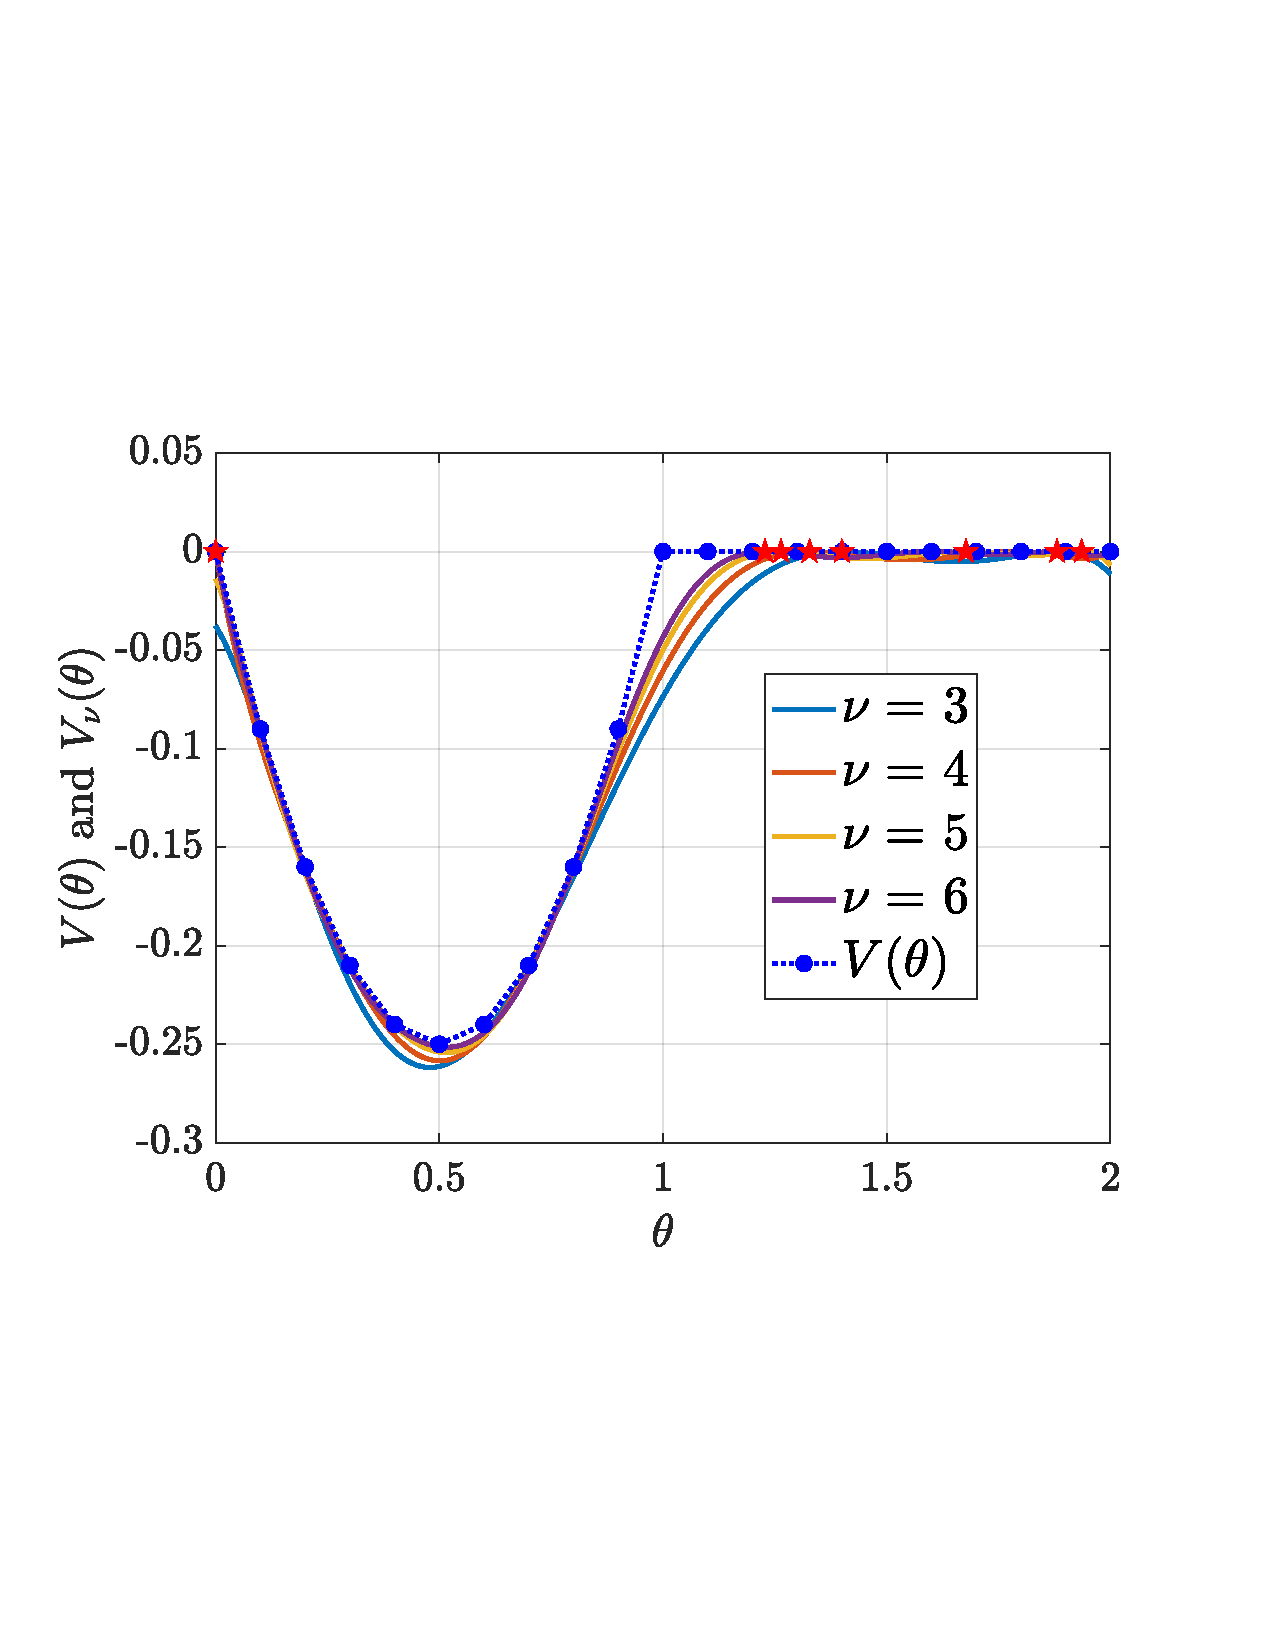
\includegraphics[width=0.65\columnwidth]{vanderpol_clean.pdf} \\
    (a) $\Theta = [0,2]$ \\

    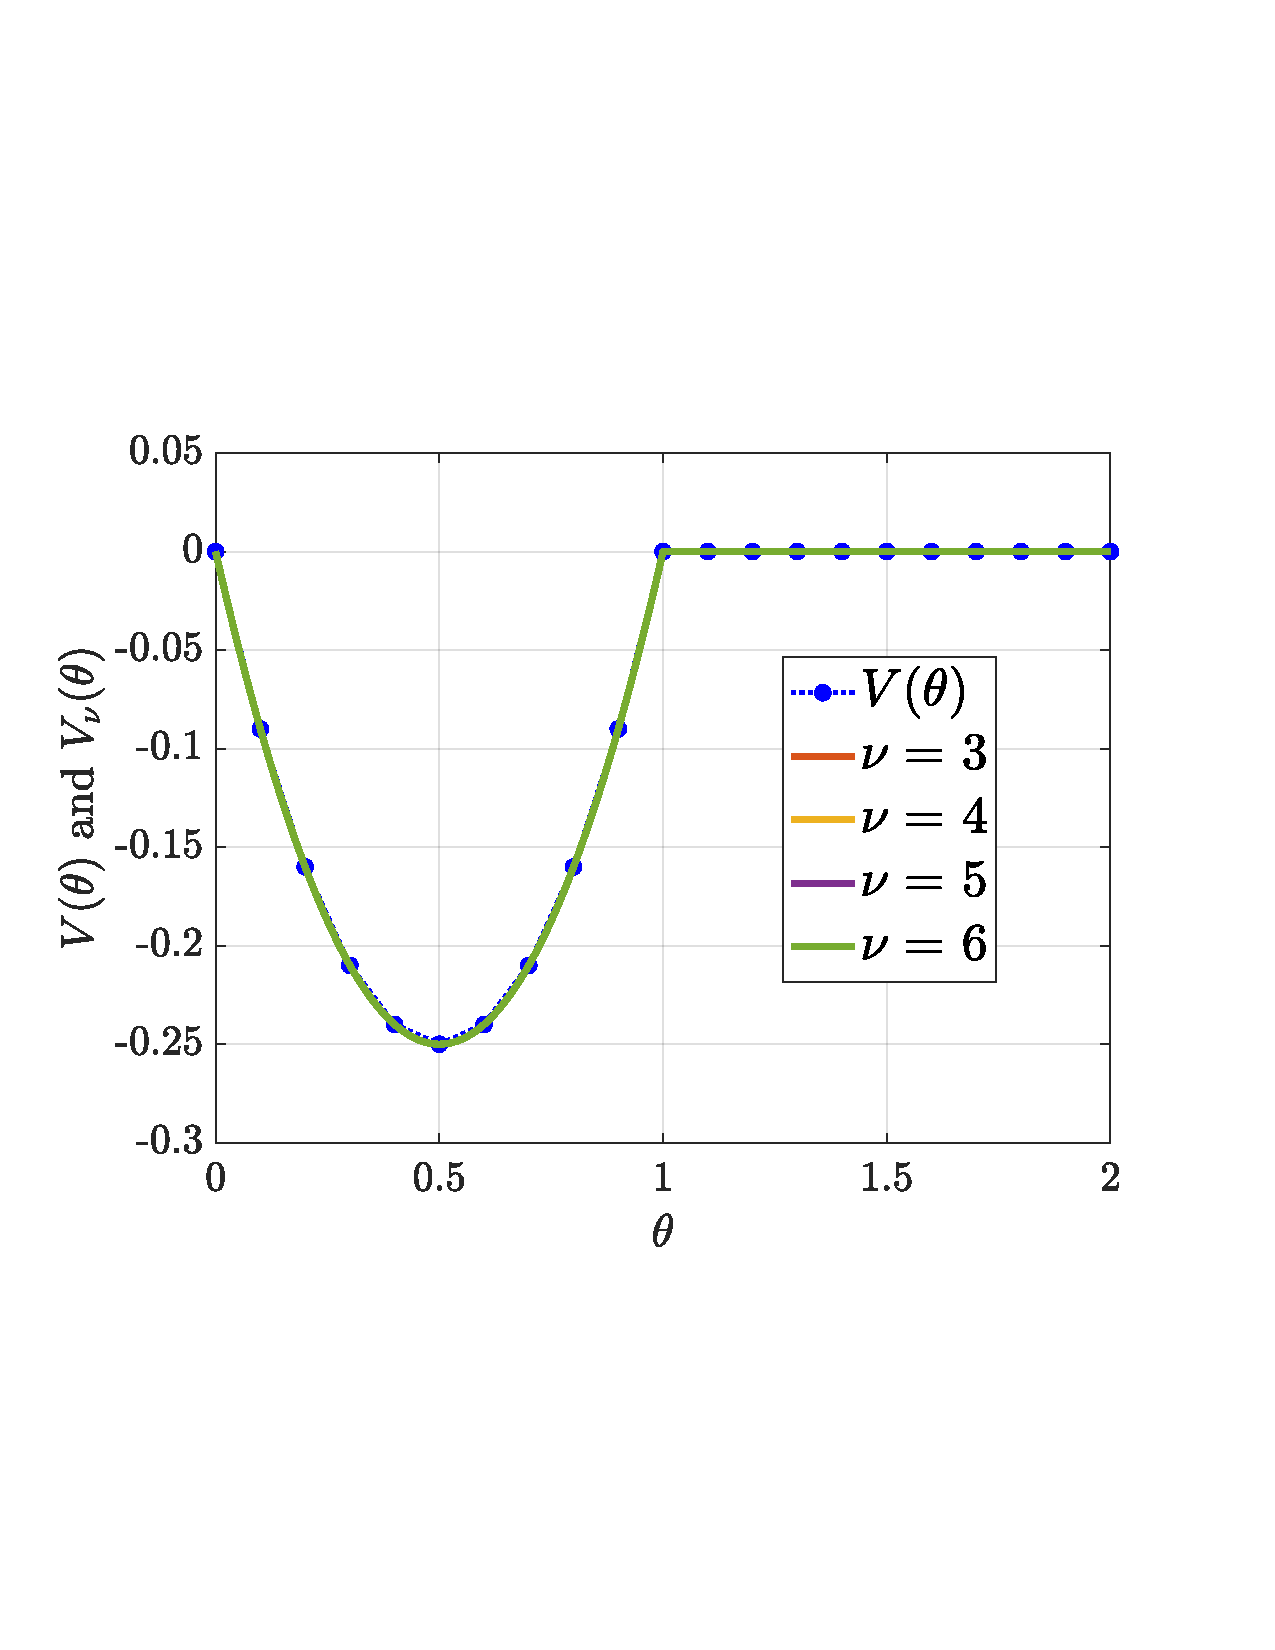
\includegraphics[width=0.65\columnwidth]{vanderpol_clean_refine.pdf} \\
    (b) $\Theta_1 = [0,1]$与$\Theta_2 = [1,2]$

    \caption{
        无不确定性的受控Van der Pol振荡器中,圆形控制障碍函数$b(x,\theta) = \theta - \parallel x \parallel^2$的验证与综合问题~\eqref{eq:cleanvdpodynamics}. 
        \label{fig:vanderpol_clean}
    }
\end{figure}


\subsection{综合问题}
我们在$\nu = 3, 4, 5, 6$处求解平方和优化问题~\eqref{eq:soslowerbound},以获得$V(\theta)$的多项式下界。附录{\color{red} DDD}中讲述了如何获得~\eqref{eq:computemoments}中的矩$\gamma_\beta$。图像~\ref{fig:vanderpol_clean}(a)中的一系列实线绘制了当$\nu = 3, 4, 5, 6$时,计算得到的$V_\nu(\theta)$。这些多项式下界很好地近似了未知的$V(\theta)$(除了$\theta = 1$附近,因为此时的$V(\theta)$不是光滑函数)。

之后我们尝试使用Lasserre's Hierarchy来最大化每一个$V_\nu(\theta)$,其中$\kappa = \nu + 2$。在 $\nu=3$ 处,我们得到 $\theta_\nu^\star = \{ 1.3997;1.8806 \}$ 和 $V_\nu^\star = \{1.2\times 10^{-8},3.2 \times 10^{-8} \}$。 在 $\nu=4$ 处,我们得到 $\theta_\nu^\star = \{ 1.3275 \}$ 和 $V_\nu^\star = \{-3.9\times 10^{-6} \}$。 在 $\nu=5$ 处,我们得到 $\theta_\nu^\star = \{ 1.2638, 1.6770, 1.9359 \}$ 和 $V_\nu^\star = \{-2.2\times 10^{-6} , -1.8 \times 10^{-6}, 8.8 \times 10^{-6} \}$。 在 $\nu=6$ 处,我们得到 $\theta_\nu^\star = \{ 0,1.2280 \}$ 和 $V_\nu^\star = \{-7.8\times 10^{-6}, - 7.4\times 10^{-8}\}$。

\subsection{精细化的综合手段}
既然我们已经知道$V(\theta)$在$\theta = 1$处不光滑,我们可以使用更为精细化的综合手段。我们对于$\Theta_1 = [0, 1]$与$\Theta_2 = [1, \theta_{\max}]$这两个区间分别计算多项式下界。图像~\ref{fig:vanderpol_clean}(b)中展示了综合生成的多项式下界$V_\nu(\theta)$(我们将$\Theta_1$与$\Theta_2$中的两个曲线联通了)。可以看到,这些下界变成了紧下界!

在一维的$V(\theta)$的验证和综合问题中,我们展示了我们算法框架的流程。有了这些认知,我们可以进一步求解具备加性不确定性的受控Van der Pol振荡器的验证与综合问题。

\section{具备加性不确定性的受控 Van der Pol 振荡器}
\label{sec:uncertainvanderpol}

下面考虑带不确定性的系统~\eqref{eq:cleanvdpodynamics}
\begin{equation}\label{eq:vdpodynamics}
    \dot{x} = \left[ \begin{array}{c}
        \dot{x}_1 \\ \dot{x}_2
    \end{array} \right] 
    = \left[ \begin{array}{c}
        x_2 \\
        \frac{1}{2}(1 - x_2^2) x_2 - x_1
    \end{array} \right]
    + \left[ \begin{array}{c}
        0 \\ x_1
    \end{array} \right] u
    + \left[ \begin{array}{c}
        0 \\ 1
    \end{array} \right] \epsilon
\end{equation}
其中,$\mathbb{U}$的定义与~\eqref{eq:cleanvdpou}中一致。

我们考虑与~\eqref{eq:cleanvdpocbf}中一样的圆形的控制障碍函数,并且在此基础上考虑验证与综合问题。然而,正如我们在章节~\ref{sec:cleanvanderpol}中看到的,在边界$\partial \mathcal{C}$上,$\dot{b}(x, \theta)$的最大值是$0$,亦即,对于综合问题~\eqref{eq:cbfsynthesis},$V^\star = 0$。这对含有不确定的系统也同样成立。

\begin{proposition}\label{prop:wrongvdpocbf}
    对于系统~\eqref{eq:vdpodynamics}和(候选的)圆形控制障碍函数~\eqref{eq:cleanvdpocbf},对于任意的$\theta \in \Theta$,有$V(\theta) \le 0$。
\end{proposition}
\begin{proof}
    见附录{\color{red} DDD}。
\end{proof}

那么,我们是否能找到一个鲁棒的控制障碍函数,使得$V(\theta)$的值严格为正呢?答案是肯定的。

现在让我们考虑椭圆形的鲁棒控制障碍函数候选者:
\begin{equation}\label{eq:ellipsoidalcbf}
    b(x, \theta) = 1 - x^T \underbrace{
        \left[ \begin{matrix}
            \theta_1 & \theta_3 \\
            \theta_3 & \theta_2
        \end{matrix} \right]
    }_{:= A} x
\end{equation}
其中它的参数空间定义为
\begin{equation}\label{eq:ellipsoidalparam}
    \Theta := \left\{ 
        \theta \in \mathbb{R}^3 \mid \theta_1, \theta_2 \in [\underline{\theta}, \overline{\theta}]^2, \theta_3^2 \le \xi^2 \theta_1 \theta_2
     \right\}
\end{equation}
其中$0 < \underline{\theta} < \overline{\theta}$且$0 < \xi < 1$。明显地,$A \succ 0$对$(\theta_1, \theta_2, \theta_3) \in \Theta$都成立。且$b(x, \theta)$定义了椭球的边界。更进一步地,假设~\ref{assume:archimedeanness}成立————附录{\color{red} DDD}证明了这一点:其计算了多项式优化问题~\eqref{eq:verifypop}中$y$的界。s使用这个函数族,我们将获得$V(\theta) > 0$。

\subsection{综合问题}
对于验证问题,此处不像章节~\ref{sec:cleanvanderpol}那么方便。这是因为对于一维的$\theta$,我们可以通过均匀采样来使得我们的样本覆盖整个参数空间$\Theta \in [0, \theta_{\max}]$。然而,若要覆盖参数空间~\eqref{eq:ellipsoidalparam},我们则需要采样更多的样本。因此,此处我们选择直接综合多项式下界。所选参数如下:$u_{\max} = 5, M_\epsilon = 0.1, \underline{\theta} = 0.25, \overline{\theta} = 0.75, \xi = 0.6$。(1)$\nu = 3$时,如图像~\ref{fig:vanderpol_uncertain}(a)所示,我们稠密地在$\left\{ \theta \mid V_\nu(\theta) \ge 0 \right\}$内采样,色彩图显示了$\Theta$内有大量的点(如图中黄色的点),使得$V_\nu(\theta)$严格大于$0$。特别地$V_\nu(\theta)$的全局最优解在$\theta^\star_\nu = [0.2500;0.2757;0.1323]$处取得,其值为$V^\star_\nu = 0.2376$。(2)图像~\ref{fig:vanderpol_uncertain}(b)展示了$\nu = 4$时的散点图。我们可以看到,能够被验证的椭圆形的鲁棒控制障碍函数的集合变得更大了。$V_\nu(\theta)$的全局最优解在$\theta^\star_\nu = [0.3278;0.2500;0.1718]$处取得,其值为$V^\star_\nu = 1.0606$。

\subsection{最大与最小椭圆}
如果我们想找这样一个椭圆形鲁棒控制障碍函数:它能够围成面积最小的椭圆————我们该怎么做呢?我们求解
\begin{equation}
    \max_{\theta \in \Theta} \left\{ \text{det}A = \theta_1 \theta_2 - \theta_3^2 \mid V_\nu(\theta) \ge 0 \right\}
\end{equation}
在$\nu = 3, \kappa = 4$时优化上式,我们能够还原出最好的一组参数:$\theta_1=0.4714,\theta_2=0.5236,\theta_3 = 0.0893$。类似地,$\theta_1=0.25,\theta_2=0.25,\theta_3 = 0.15$最小化了$\text{A}$,亦即,其最大化了椭圆面积。


%!TEX root = ../thuthesis-example.tex
\begin{figure}
    \centering
    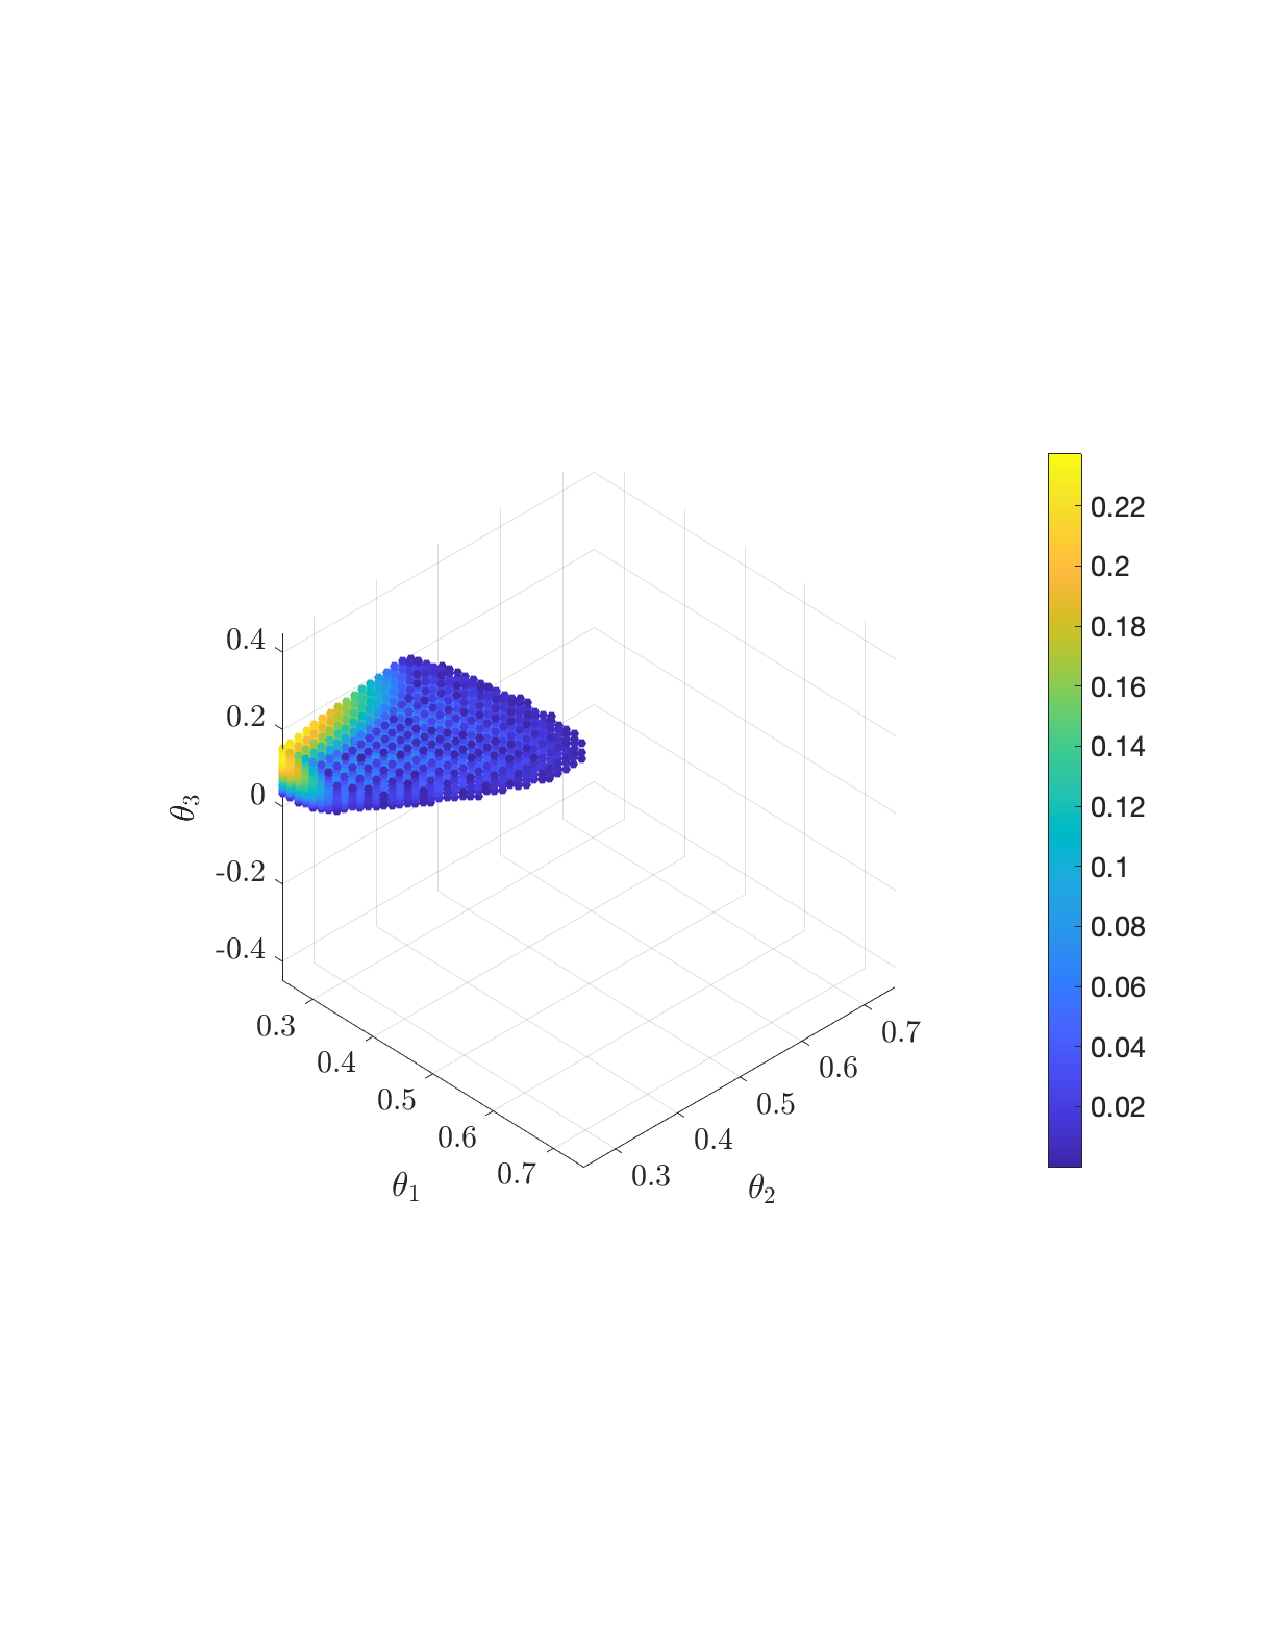
\includegraphics[width=0.8\columnwidth]{vanderpol_uncertain_theta_v3.pdf} \\
    (a) $\nu = 3$ \\

    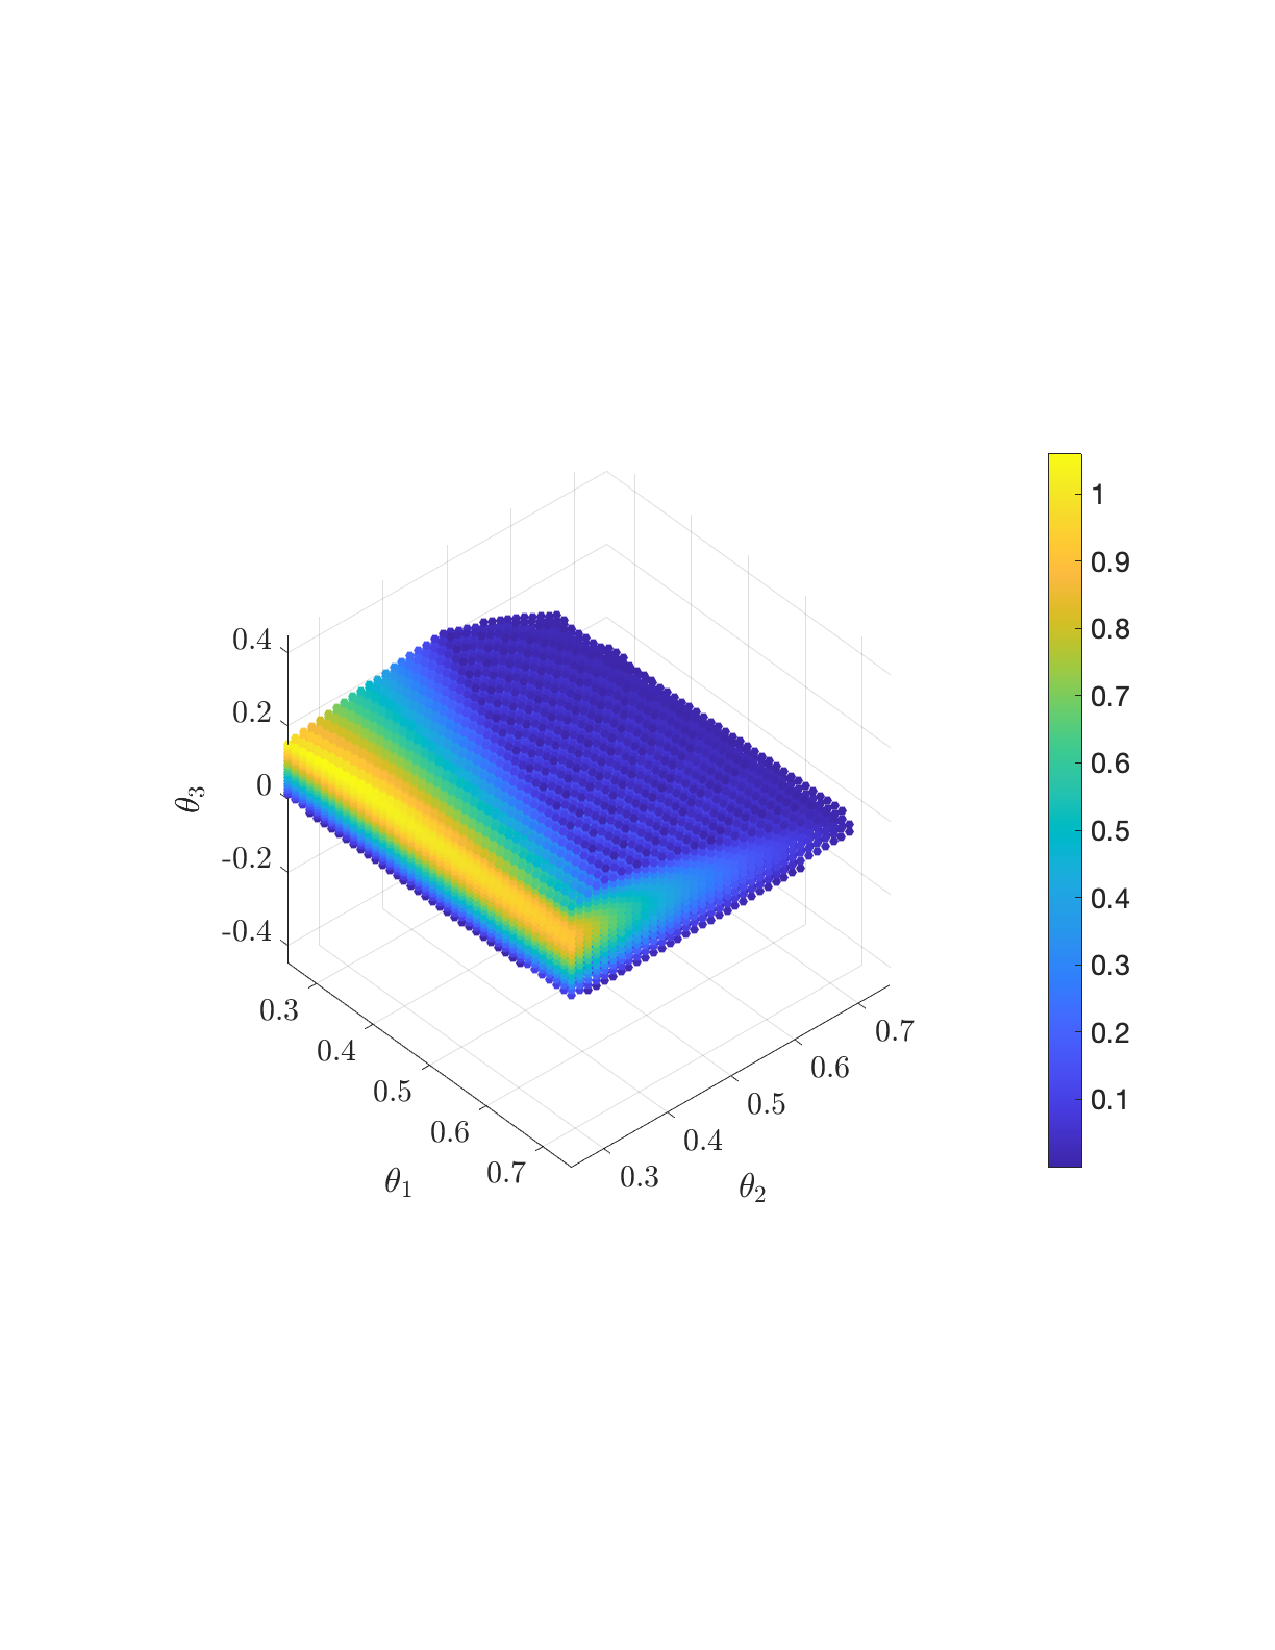
\includegraphics[width=0.8\columnwidth]{vanderpol_uncertain_theta_v4.pdf} \\
    (b) $\nu = 4$

    \caption{
        无不确定性的受控Van der Pol振荡器中~\eqref{eq:vdpodynamics},椭圆形控制障碍函数$b(x,\theta) = 1 - x^T A x$所对应的综合问题。
        \label{fig:vanderpol_uncertain}
    }
\end{figure}

% % !TeX root = ../thuthesis-example.tex

\chapter{总结}

本文中,我们将鲁棒控制障碍函数的验证与综合问题转化为了多层次多项式优化问题。我们使用的KKT条件将内部连两级优化做了闭式求解,最终将验证问题转化成了单级多项式优化问题,将综合问题转化成了最小-最大多项式优化问题。我们涉及了多级半正定优化来近似解决上述两种多项式优化问题,并且取得了渐进的全局收敛性的理论保证。我们还对多控制障碍函数问题进行了输入研究。我们再受控Van der Pol振荡器上验证了我们的算法。未来,我们打算将我们的方法扩展至多控制障碍函数问题上。


% 其他部分
\backmatter

% \listoffigures           % 插图清单
% \listoftables            % 附表清单

% 参考文献
\bibliography{ref/refs}  % 参考文献使用 BibTeX 编译
% \printbibliography       % 参考文献使用 BibLaTeX 编译

% 附录
% 本科生需要将附录放到声明之后,个人简历之前
% \appendix
% \input{data/appendix-survey}       % 本科生:外文资料的调研阅读报告
% % !TeX root = ../thuthesis-example.tex

% \usepackage{amsmath,amsfonts}
% \usepackage{multicol}
% \usepackage{graphicx}

%definitions
\renewcommand{\AA}{{\cal{A}}}
\newcommand{\II}{{\cal{I}}}
\newcommand{\CC}{{\cal{C}}}
\newcommand{\FF}{{\cal{F}}}
\newcommand{\LL}{{\cal{L}}}
\newcommand{\R}{\mathbb{R}}
% \newcommand{\N}{\mathbb{N}}
\renewcommand{\SS}{{\cal{S}}}
\newcommand{\TT}{{\cal{T}}}
\newcommand{\UU}{{\mathbf{U}}}
\newcommand{\XX}{{\mathbf{X}}}
\newcommand{\I}{{\boldsymbol{1}}}
\def\z{\mathbf{z}}
\def\w{\mathbf{w}}
\def\y{\mathbf{y}}
\def\K{\mathbf{K}}
\newcommand{\comment}[1]{\textcolor{red}{\textbf{#1}}}

% \newtheorem{assumption}{Assumption}
% \newtheorem{example}{Example}
% \newtheorem{remark}{Remark}

\begin{translation}
\label{cha:translation}

\title{标题:通过占据测度实现非线性最优控制综合}
\author{Didier Henrion, Jean B. Lasserre and Carlo Savorgnan}
\maketitle

\begin{abstract}
  我们考虑所有问题数据都是多项式的非线性最优控制问题 (OCP)。 在本文的第一部分,我们回顾了如何使用线性矩阵不等式 (LMI) 松弛的层次结构,使用占用度量逐点逼近给定 OCP 的最优价值函数。 在第二部分中,我们将方法扩展到在给定集合上逼近最优值函数,并使用这样的函数来建设性和计算性地推导出几乎最优的控制律。数值例子表明了该方法的有效性。
\end{abstract}

\section{引言}

众所周知,尽管 Pontryagin 最小原理和 Hamilton-Jacobi-Bellman 最优条件等理论工具的强大功能,解决最优控制问题 (OCP) 可能是一项非常艰巨的任务。
在处理状态和输入约束时,这种说法尤其正确。


\textbf{贡献。} 在本文中,我们考虑所有问题数据都是多项式的 OCP 类。
我们部署的方法(在 \cite{LasPriHen2005} 中引入)基于矩理论,包括推导 OCP 的凸线性矩阵不等式 (LMI) 松弛的层次结构,它给出最优值下限的递增序列 . 这些 LMI 问题可以使用现成的半定规划 (SDP) 求解器来解决。

关于 \cite{LasPriHen2005} 及其扩展版本 \cite{LasHenPriTre2008} 的贡献是双重的。 首先,从基本概念开始,以更简单的方式获得松弛的推导。 第二个也是更重要的贡献是,我们展示了如何应用该方法来近似集合上的最优值函数,并以建设性和计算方式推导
一个控制律。 几个简单的例子说明了这种方法。

\textbf{符号。}
$\R$ 和 $\mathbb{N}$ 分别表示实数集和整数集。
$\R[y]=[y_1, \dots , y_n]$ 表示变量 $y$ 中的多项式环。
$\R[y]_d=[y_1, \dots , y_n]$ 表示变量 $y$ 中次数最多为 $d$ 的多项式环。
当 $y \in \R^n$ 和 $\alpha\in\mathbb{N}^n$ 时,$y^\alpha$ 代表 $y_1^{\alpha_1} \dots y_n^{\alpha_n}$。
给定一个多项式函数 $\varphi$,$\deg(\varphi)$ 是其单项式的最大次数。
给定一个可微函数 $\varphi(y)$, $\nabla_y(\varphi)=[\frac{\partial\varphi}{\partial y_1}, \dots ,\frac{\partial\varphi}{\partial y_n }]$ 是它相对于 $y$ 的梯度。
$\delta_{y_0}$ 是 $y_0$ 处的狄拉克测度。
$v'$ 表示 $v$ 的转置。

\section{问题定义}
考虑由微分方程描述的连续时间系统
\begin{equation}\label{eq:dynamics}
\dot x(t) = f(t, x(t), u(t))
\end{equation}
其中 $x\in\R^n$ 和 $u\in\R^m$ 分别是状态向量和输入向量。
通过定义代价函数
\begin{equation}\label{eq:cost}
\int_0^T h(t, x(t), u(t)) dt + H(x(T))
\end{equation}
初始约束为
\begin{equation}\nonumber
x(0) \in \CC_I=\{ x: g_{I_j}(x)\leq 0, ~ j=1,\dots,n_I \} 
\end{equation}
末态约束为
\begin{equation}\nonumber
x(T) \in \CC_F=\{ x: g_{F_j}(x)\leq 0, ~ j=1,\dots,n_F \}
\end{equation}
我们可以制定几个OCP。 例如,当 $\CC_I$ 和 $\CC_F$ 仅包含一个点时,我们遇到了将系统从指定的初始条件 $x(0)=x_0$ 驱动到最终条件 $x(T)=x_T$ 的经典问题 通过最小化给定的成本。

在续集中,我们将考虑在轨迹 $(t, x(t), u(t)) \in \CC_T$ 上附加约束的所有问题,其中
\begin{equation}\nonumber
\CC_T=\{ (t,x,u): g_{T_j}(t,x,u)\leq 0, ~ j=1,\dots,n_T \}.
\end{equation}

推导该方法所必需的一个重要假设是所有问题数据都是多项式的。 更确切地说:
\begin{assumption}\label{as:poly}
  函数 $f$、$h$、$H$、$g_{I_j}$、$g_{T_j}$ 和 $g_{F_j}$ 是多项式的。
\end{assumption}

\section{最优控制的矩方法}
矩方法的关键思想是定义三个 \textit{占用度量},它们传达有关系统初始条件、轨迹和最终条件的信息。
然后根据此类措施的时刻对 OCP 进行重新措辞。
得到的凸问题包含三个成分:
\begin{itemize}
\item 一组对表征系统动力学的矩的线性等式约束;
\item 一组半定约束,这些约束来自矩属于一个度量的事实;
\item 一组半定约束,它们将 $\CC_I$、$\CC_T$ 和 $\CC_F$ 引起的约束转换到测度的支持上。
\end{itemize}
为了得出这个约束,我们假设地平线 $T$ 是固定的。


\subsection{轨迹约束}
为了获得轨迹约束,我们从系统轨迹可以表征研究某些\textit{测试函数}如何沿着轨迹演变的想法开始。 为此,我们选择 $t^\alpha x^\beta$ 形式的单项式函数。 考虑轨迹 $x(t)$。 使用微积分基本定理我们可以写为
\begin{equation}\label{eq:ftoc}
T^\alpha x(T)^\beta = 0^\alpha x(0)^\beta + \int_0^T \frac{d(t^\alpha x(t)^\beta)}{dt} dt.
\end{equation}
轨迹约束是通过重新表述方程 (\ref{eq:ftoc}) 获得的
三个适当定义的占据测度。

\textit{最终占据测度} $\mu_F$ 捕获了时间 $T$ 的状态信息
\begin{equation}\nonumber
x(T)^\beta = \int x^\beta \delta_{x(T)}(dx) = \int x^\beta d\mu_F.
\end{equation}
\textit{初始占据测度} $\mu_I$ 捕捉系统初始状态的信息
\begin{equation}\nonumber
x(0)^\beta = \int x^\beta \delta_{x(0)}(dx) = \int x^\beta d\mu_I.
\end{equation}
\textit{轨迹占据测度} $\mu_T$ 捕获了关于 $t$, $x(t)$ 和 $u(t)$ 沿轨迹的值的信息
\[
\int_0^T \!\! t^\gamma x(t)^\eta u(t)^\nu dt \!
=\!\int_0^T \!\!\!\!\int t^\gamma x^\eta u^\nu \delta_{x(t),u(t)}(dx,du)dt \!
=\!\int x^\gamma u^\eta t^\nu d\mu_T.
\]
请注意 $\mu_F$ 和 $\mu_I$ 是概率度量,它们的质量等于 $1$。

接下来,如果 $f\in\R[t,x,u]$ 那么 $\frac{d(x^\alpha t^\beta)}{dt}\in\R[t,x,u]$ 因为
\begin{equation}\nonumber %\label{aux}
\frac{d(x^\alpha t^\beta)}{dt} \! = \! \frac{\partial(x^\alpha t^\beta)}{\partial t} + \nabla_x (x^\alpha t^\beta)f(x,u) \! = \!\! \sum_{\gamma,\eta,\nu} \! a^{\alpha\beta}_{\gamma\eta\nu} x^\gamma u^\eta t^\nu
\end{equation}
对于某些依赖于 $f$ 的系数 $a^{\alpha\beta}_{\gamma\eta\nu}$。
导数的次数是$\deg(x^\alpha t^\beta)-1+\deg(f)$。
使用前面的等式,(\ref{eq:ftoc}) 可以改写为
\begin{equation}\label{eq:meascons}
%= 0^\alpha \int x^\beta d\mu_I + \int \frac{(t^\alpha x^\beta)}{dt} d\mu_T \\
T^\alpha \int x^\beta d\mu_F 
= 0^\alpha \int x^\beta d\mu_I + \sum_{\gamma,\eta,\nu} a^{\alpha\beta}_{\gamma\eta\nu} \int t^\gamma x^\eta u^\nu d\mu_T,
\end{equation}
即,时刻之间的{\it 线性}关系
$\mu_F, \mu_I$ 和 $\mu_T$。
即,引入符号 
$z_{\beta}=\int x^\beta d\mu_F$,
$w_{\beta}=\int x^\beta d\mu_I$,
$y_{\gamma\eta\nu}=\int t^\gamma x^\eta u^\nu d\mu_T$, 
我们得到
\begin{equation}\label{eq:momcons}
T^\alpha z_{\beta} = 0^\alpha w_{\beta} + \sum_{\gamma,\eta,\nu} a^{\alpha\beta}_{\gamma\eta\nu} y_{\gamma\eta\nu}
\end{equation}
对于每个 $\alpha,\beta\in\mathbb{N}\times\mathbb{N}^{n}$。 请注意,从 (\ref{eq:momcons}),
$\mu_T$ 的质量是 $T$。
在紧凑的表示法中,考虑次数高达 $r$ 的测试函数和次数最多为 $r$ 的单项式的规范基础:
\begin{equation}\nonumber
m_r(x)=[1,x_1,\dots,x_n,x_1^2,x_1x_2,\dots,x_1^r,x_1^{r-1}x_2,\dots,x_n^r]'.
\end{equation}
定义向量
$\z_r=\int m_r(x) d\mu_F$,
$\w_r=\int m_r(x) d\mu_I$和
$\y_k=\int m_k(t,x,u) d\mu_T$.
Then,
\begin{equation}\label{eq:momcon}
A_F \z_r = A_I \w_r + A_T \y_k
\end{equation}
其中 $k\geq r-1+\deg(f)$ 和矩阵 $A_F$、$A_I$ 和 $A_T$ 的系数可以从等式 (\ref{eq:momcons}) 中获得。

将系数向量 $c_h$ 和 $c_H$ 定义为
\begin{equation}\nonumber
h(t,x,u)=c_h'm_k(x,t,u), \qquad H(x)=c_H' m_r(x).
\end{equation}
观察到
\begin{equation}\label{criterion}
\int_0^T h(t, x(t), u(t)) dt + H(x(T))=c_h' \y_k+  c_H' \z_r,
\end{equation}
即,OCP 的标准是 $\z_r$ 和 $\y_k$ 上的线性泛函。

到目前为止,对于给定的轨迹 $x(t)$,我们已经描述了三个相关占据测度的时刻满足的线性约束。 现在,如果轨迹未知,则三个度量未知,我们可以考虑抽象线性规划 (LP) 问题 $J(\mu_I) = \min_{\mu_T,\mu_I,\mu_F}
\int h d\mu_T + \int H d\mu_F$
受 (\ref{eq:meascons}) 影响,其目的是找到与最佳轨迹相关的占据测度。 $\mu_F$, $\mu_I$, $\mu_T$ 的特征是通过它们各自的截断矩向量 $\z_r$, $\w_r$, $\y_k$,
剩下的困难是找到条件,确保这些向量和测量的力矩向量分别支持 $\CC_F$、$\CC_I$、$\CC_T$。 这将在下一节中解释。

该方法的一个很好的特点是我们可以使用初始和最终措施。 例如,如果 $\mu_I=\delta_{x_0}$,我们检索具有固定初始状态 $x_0$ 的 OCP 的最优成本 $J(\delta_{x_0})$。 现在,如果 $\mu_I$ 未知,但已知支持 $\CC_I$,则 $J(\mu_I)=\min_{x_0\in\CC_I}J(\delta_{x_0})$。 最后,如果 $\mu_I$ 已知,但狄拉克未知,则求解上述 LP 问题旨在计算 $\int J(\delta_{x_0})d\mu_I(x_0)$。

\subsection{矩矩阵约束}
存在线性规划 (LP) 或半定规划 (SDP) 无限向量是 {\it moment} 向量的充分必要条件,即紧基本半代数集上某个有限 Borel 测度的矩向量 ; 参见例如 \cite{Put1993}。 我们选择了后者,因为它已被证明对数值目的更有效 \cite{LasPri2004}。

$r$ 为偶数,令
\begin{equation}\nonumber
M(\z_r)=\int m_{r/2}(x) m_{r/2}(x)' d\mu_F
\end{equation}
是与 $\mu_F$ 关联的 $r$ 阶 {\it 矩矩阵}。 显然,$M(\z_r)$是半正定的,记为$M(\z_r)\succeq0$。 因此,在 OCP 的凸弛豫中,施加
\begin{equation}\label{eq:mmc}
M(\z_r) \succeq 0,
\end{equation}
并且对 $\w_r$ 和 $\y_k$ 施加了类似的约束。

\subsection{定位矩阵约束}
与上一小节类似,可以根据 $\z_r、\w_r$ 和 $\y_k$ 上的线性矩阵不等式表示由 $\CC_I$、$\CC_T$ 和 $\CC_F$ 引起的支持约束。 为了推导出这样的不等式,定义
\begin{equation}\nonumber
d_{F_j}=\left\{
\begin{array}{ll}
\deg(g_{F_j}(x)) & \mbox{if}~\deg(g_{F_j}(x))~\mbox{is even} \\
\deg(g_{F_j}(x))+1 & \mbox{if}~\deg(g_{F_j}(x))~\mbox{is odd}
\end{array} \right.
\end{equation}
和定位矩阵
\begin{equation}\nonumber
L_{g_{F_j}}(\z_r)=\int g_{F_j}(x) m_{(r-d_{F_j})/2}(x) m_{(r-d_{F_j})/2}(x)' d\mu_F.
\end{equation}
矩阵 $g_{F_j}(x) m_{(r-d_{F_j})/2}(x) m_{(r-d_{F_j})/2}(x)'$ 对于每个值都是半正定的 $x$ 使得 $g_{F_j}(x)\geq 0$。 因此,如果 $\mu_F$ 在 $\CC_F$ 上得到支持,则 $L_{{F_j}}(\z_r)\succeq0$ 对于每个 $j$ 因此,在 OCP 的凸松弛中,施加半定约束
\begin{equation}\label{eq:lmc}
L_{g_{F_j}}(\z_r) \succeq 0 \qquad j=1,\dots,n_F
\end{equation}
以及 $\w_r$ 和 $\y_k$ 的类似半定约束。

有关力矩和局部化矩阵约束的更多详细信息,请参见 \cite{Las2001}。

\subsection{凸松弛}
为了构造 OCP 的凸松弛,设 $r$ 和 $k$ 为偶数,使得
\begin{equation}\nonumber
r\geq\deg(H), \quad k\geq\deg(h), \quad k\geq r+\deg(f).
\end{equation}
在本文中,我们将假设初始概率
测量 $\mu_I$ 通过其矩 $\w_r$ 已知。

凸松弛是以下截断矩问题:
\begin{equation}\label{eq:momocp2}
\begin{split}
\min_{\z_r, \y_k}\quad & c_h' \y_k+  c_H' \z_r \\
& A_F \z_r = A_I \bar \w_r + A_T \y_k \\
& M(\z_r)\succeq 0, ~~ L_{g_{F_j}}(\z_r)\succeq 0, ~~ \forall j=1,\dots,n_F \\
& M(\y_k)\succeq 0, ~~ L_{g_{T_j}}(\y_k)\succeq 0, ~~ \forall j=1,\dots,n_T
\end{split}
\end{equation}
其中符号 $\bar \w_r$ 表示力矩向量是已知的。
当下问题应注意两个重要事实 (\ref{eq:momocp2}):
\begin{itemize}
  \item 对力矩的约束对应于必要条件,因此,
  通常,人们只能获得 OCP 最优值的下限;
  \item with $\hat r > r$ and $\hat k > k$,$r$ and $k$ 的原始问题的约束是 $\hat r$ and $\hat{k}$。 因此,增加 $r$ 和 $k$ 的值会产生最优值下限的单调非递减序列。
  \end{itemize}

\begin{remark}
  如果初始测量 $\mu_I$ 未知,我们将不得不包括额外的约束 $M(\w_r)\succeq 0$, $L_{g_{I_j}}(\w_r)\succeq 0$, $\forall j=1,\dots,n_I$ 现在 $\w_r$ 是一个未知的力矩向量,第一个条目等于 1。
\end{remark}

\begin{remark}
  本文的目标之一是从真正基本的概念出发推导 OCP 的凸松弛。 使用紧集 $\K$ 上有界连续函数的 Banach 空间与 $\K$ 上的有限符号 Borel 测度的 Banach 空间之间的对偶性作为起点,也可以获得相同的优化问题,如 \cite{LasPriHen2005,LasHenPriTre2008},其中最优值的下限序列显示在问题数据的某些假设下收敛。 感兴趣的读者可以参考这些论文以了解更多详细信息。
\end{remark}

\section{总结}

本文是 \cite{LasPriHen2005,LasHenPriTre2008} 的后续论文,其中根据占用度量方法推导了多项式最优控制问题 (OCP) 的最优值的下限序列。 在当前的论文中,我们提出了一些技术,可以从 OCP 的凸线性矩阵不等式 (LMI) 松弛的解中建设性地推导出控制律。 因此,我们的贡献可以看作是对 \cite{LasPriHen2005,LasHenPriTre2008} 性能分析结果综合的扩展。

一般来说,我们认为 OCP 的矩公式是基于 Lyapunov 或 Hamilton-Jacobi-Bellman 技术的间接方法的一种有吸引力的替代方法。 力矩公式直接处理系统轨迹。 由此产生的原始 LMI 矩问题承认对偶 LMI 平方和 (SOS) 公式,但是,它有助于显式计算控制律。 在这种情况下,泛函分析(测度论)和代数几何(半代数正多项式的表示)之间的良好相互作用可以为潜在的困难控制综合问题提供建设性的答案。

该方法的当前局限性如下。

首先,当我们正在寻找一个多项式值函数(Hamilton-Jacobi-Bellman 方程的平滑子解)时,它近似于(可能是非平滑的)最优值函数 $\bar{\varphi}(t,x)$,它 可能会发生精度在 $\bar{\varphi}(t,x)$ 不平滑的点处恶化的情况。 沿着最优轨迹移动的邻域中的状态空间划分和/或多项式值函数的迭代计算可以帮助解决这个问题,但代价是增加了计算负担。

其次,我们依赖于当前可用的通用 SDP 求解器的性能。 半定规划是一个相对年轻的研究领域,SDP 求解器的成熟度远不及线性或凸二次规划求解器。 更具体地说,据我们所知,目前没有数值稳定的 SDP 求解器,也没有易于处理的 LMI 问题条件估计。 例如,预计选择表示多项式和矩的基会对问题条件产生重大影响,从而影响求解器的数值行为。

第三,LMI 问题中的变量和约束的数量随着状态和输入变量的数量以及价值函数的多项式逼近度的函数而快速增长。 当前的通用 SDP 求解器可以处理数千个变量和约束,远低于对应于具有 6 个状态和 2 个输入的 OCP 的矩 LMI 问题的维度。 出于这些原因,专门针对矩 LMI 问题的拟 Hankel 或拟 Toeplitz 结构量身定制的专用原始对偶内点方法将受到欢迎。

最后,我们目前正在为 GloptiPoly 3 \cite{HenLasLof2007} 开发一个用户友好的 OCP 模块,这有助于明确地将 OCP 表述为广义矩问题。 用户只需提供OCP的多项式数据,模块自动生成近似最优控制律。 一旦准备就绪并完整记录,该软件将可从 GloptiPoly 3 网页免费下载。

% \tableofcontents


% 本科生的外文资料书面翻译。


% \section{图表示例}

% \subsection{图}

% 附录中的图片示例(图~\ref{fig:appendix-translation-figure})。

% \begin{figure}
%   \centering
%   \includegraphics[width=0.6\linewidth]{example-image-a.pdf}
%   \caption{附录中的图片示例}
%   \label{fig:appendix-translation-figure}
% \end{figure}


% \subsection{表格}

% 附录中的表格示例(表~\ref{tab:appendix-translation-table})。

% \begin{table}
%   \centering
%   \caption{附录中的表格示例}
%   \begin{tabular}{ll}
%     \toprule
%     文件名          & 描述                         \\
%     \midrule
%     thuthesis.dtx   & 模板的源文件,包括文档和注释 \\
%     thuthesis.cls   & 模板文件                     \\
%     thuthesis-*.bst & BibTeX 参考文献表样式文件    \\
%     thuthesis-*.bbx & BibLaTeX 参考文献表样式文件  \\
%     thuthesis-*.cbx & BibLaTeX 引用样式文件        \\
%     \bottomrule
%   \end{tabular}
%   \label{tab:appendix-translation-table}
% \end{table}


% \section{数学公式}

% 附录中的数学公式示例(公式\eqref{eq:appendix-translation-equation})。
% \begin{equation}
%   \frac{1}{2 \uppi \symup{i}} \int_\gamma f = \sum_{k=1}^m n(\gamma; a_k) \mathscr{R}(f; a_k)
%   \label{eq:appendix-translation-equation}
% \end{equation}


% \section{文献引用}

% 文献引用示例\cite{abrahams99tex}。


% \appendix

% \section{附录}

% 附录的内容。


% % 书面翻译的参考文献
\bibliographystyle{unsrtnat}
\bibliography{ref/appendix}

% % 书面翻译对应的原文索引
% \begin{translation-index}
%   \nocite{salomon1995advanced}
%   \bibliographystyle{unsrtnat}
%   \bibliography{ref/appendix}
% \end{translation-index}


\end{translation}
  % 本科生:外文资料的书面翻译
% % !TeX root = ../thuthesis-example.tex

\chapter{补充内容}

\section{性质~\ref{prop:boundeddual}的证明}
\label{app:proof:prop:boundeddual}

\begin{proof}
  (1)考虑$\mathbb{U}$是一个多面体,且其没有退化的极值点。观察可得,“$\max_{u \in \mathbb{U}} L_gb(x, \theta) u$”是一个关于$u$的线性函数(当$(x, \theta)$固定的时候)。由于$\mathbb{U}$没有退化的极值点,在最优解$u^\star$处,必有$m' \le m$个线性无关的约束被激活。因此,共有$m'$个非零的$\zeta_i^\star$~\cite{bertsimas97book-lp}。不失一般性地,我们假设$i = 1, \dots, m'$为被激活的约束。则KKT的stationary条件~\eqref{eq:kktstationary}可以被表示为:
  \begin{eqnarray}
    \underbrace{
      \left[ \begin{matrix}
        w_1 & \cdots & w_{m'}
      \end{matrix} \right]
    }_{:= W \in \mathbb{R}^{m \times m'}} = L_gb(x, \theta)
  \end{eqnarray}
  而这暗含了$(\zeta^\star)^T (W^TW) (\zeta^\star) = \parallel L_gb(x, \theta) \parallel^2$。当$W^TW \succ 0$时(亦即,$\left\{ w_i \right\}_{i=1}^{m'}$线性无关),我们有
  \begin{eqnarray}
    \left\lVert \zeta^\star \right\rVert \le \frac{
      \left\lVert L_gb(x, \theta) \right\rVert^2
    }{
      \lambda_{\min} (W^T W)
    }
  \end{eqnarray}
  最后,我们观察到$\left\lVert L_gb(x, \theta) \right\rVert^2$是有界的。这是因为它在紧集$\partial \mathcal{C} \times \Theta$上是光滑的。因此,$\left\lVert \zeta^\star \right\rVert^2$是有界的。

  (2)考虑$\mathbb{U}$是一个箱型,它的每一个维度的取值范围都是$[-w_i, w_i]$。如此一来,KKT条件中的complementarity条件~\eqref{eq:kktcomp}说明了以下两者中有且仅有一者成立:第一,$\zeta_i^\star = 0$;第二,$\zeta_i^\star \ne 0$,但是$u_i^\star = \pm w_i$。在第二种情形下,使用KKT条件中的stationary条件~\eqref{eq:kktstationary},我们有
  \begin{eqnarray}
    \zeta_i^\star = \frac{
      [L_gb(x, \theta)]_i
    }{2u_i^\star} \Rightarrow 
    (\zeta_i^\star)^2 = \frac{
      [L_gb(x, \theta)]_i^2
    }{4 w_i^2}, i = 1, \dots, m
  \end{eqnarray}
  其中$[L_gb(x, \theta)]_i$表示了$L_gb(x, \theta)$的第$i$项。由于$[L_gb(x, \theta)]_i$是有界的,$(\zeta_i^\star)^2$也是有界的。

  (3)现考虑$\mathbb{U}$是一个椭球,且其被一个单独的约束$u^T W u \le 1$所定义。则KKT条件的complentarity条件~\eqref{eq:kktcomp}说明了以下两者中有且仅有一者成立:第一,$\zeta^\star=0$;第二,$\zeta^\star \ne 0$,但是$(u^\star)^T W (u^\star) = 1$。在第二种条件的情况下,使用KKT条件中的stationary条件~\eqref{eq:kktstationary},我们有
  \begin{eqnarray}
    (\zeta^\star)^2 = \frac{
      \left\lVert L_gb(x, \theta) \right\rVert^2
    }{4 \left\lVert W u^\star \right\rVert^2} 
    \le \frac{
      \left\lVert L_gb(x, \theta) \right\rVert^2
    }{4 \lambda_{\min}(W)} 
  \end{eqnarray}
  由于$\left\lVert L_gb(x, \theta) \right\rVert^2$在$\partial \mathcal{C} \times \Theta$上是有界的,$(\zeta^\star)^2$在$\partial \mathcal{C} \times \Theta$上也是有界的。
\end{proof}

\section{对于系统~\eqref{eq:cleanvdpodynamics}和控制障碍函数~\eqref{eq:cleanvdpocbf},证明~\eqref{eq:standardpop}中的$y$有界}
\label{app:bound:y:cleanvdp}

明显地,$\left\lVert x \right\rVert^2 \le \theta$,$u^2 \le u_{\max}^2$是有界的。然而,我们还需要证明$\zeta^\star$是有界的。KKT条件的complentarity条件~\eqref{eq:kktcomp}说明了以下两者中有且仅有一者成立:第一,$\zeta^\star=0$;第二,$\zeta^\star \ne 0$,但是$c_{u,i}(u) = 0$,这意味着$u^\star = \pm u_{\max}$。在第二种情况下,使用KKT条件中的stationary条件~\eqref{eq:kktstationary},我们有
\begin{eqnarray}
  2\zeta^\star u^\star = L_gb(x, \theta) = -2 x_1 x_2
\end{eqnarray}
求解其中的$\zeta^\star$,我们有
\begin{eqnarray}
  \zeta = \frac{-x_1 x_2}{u^\star} \Rightarrow 
  (\zeta^\star)^2 = \frac{x_1^2 x_2^2}{u_{\max}^2} \le \frac{
    (x_1^2 + x_2^2)^2
  }{4 u_{\max}^2} = \frac{\theta_2}{4 u_{\max}^2}
\end{eqnarray}

\section{性质~\ref{prop:wrongvdpocbf}的证明}
\label{app:proofwrongvdpocbf}

\begin{proof}
  我们有
  \begin{subequations}
    \begin{eqnarray}
      L_fb(x, \theta) =& -x_2^2 (1 - x_2^2) \\
      L_gb(x, \theta) =& -2x_1 x_2 \\
      L_Jb(x, \theta) =& -2x_2
    \end{eqnarray}
  \end{subequations}
  作为结果,我们有:
  \begin{subequations}
    \begin{eqnarray}
      V_u^\star =& \displaystyle \max_{u^2 \le u_{\max}^2} (-2 x_1 x_2) u 
      = 2 u_{\max} |x_1 x_2| \\
      V_\epsilon^\star =& \displaystyle \min_{
        \left\lVert \epsilon \right\rVert \le M_\epsilon
      } -2 x_2 \epsilon 
      = -2 M_\epsilon |x_2|
    \end{eqnarray}
  \end{subequations}
  以及
  \begin{eqnarray}
    V(\theta) = \min_{\left\lVert x \right\rVert^2 = \theta} 
    -x_2^2 (1 - x_2^2) + u_{\max} |x_1 x_2| - M_\epsilon |x_2|
  \end{eqnarray}
  我们选择$x_2 = 0, x_1 = \pm \sqrt{\theta}$,可以得到$V(\theta) \le 0$。
\end{proof}

\section{对于系统~\eqref{eq:vdpodynamics}和控制障碍函数~\eqref{eq:ellipsoidalcbf},证明~\eqref{eq:standardpop}中的$y$有界}
\label{app:bound:y:uncertainvdp}

显然,$u^2 \le u_{\max}$是有界的。而$x$也是有界的,这是因为
\begin{eqnarray}
  \max_{x^T A x = 1} \overset{v := A^{1/2}x}{=} 
  \max_{v^T v = 1} v^T A^{-1} v = \frac{1}{\lambda_{\min}(A)}
\end{eqnarray}
其中$\lambda_{\min}$和$\lambda_{\max}$表示了$A$的特征值中的最大值和最小值。注意到
\begin{eqnarray}
  \lambda_{\min} (\lambda_{\max} + \lambda_{\min}) \ge \lambda_{\min} \lambda_{\max} = \theta_1 \theta_2 - \theta_3^2 \Rightarrow \\
  \lambda_{\min} \ge \frac{
    \theta_1 \theta_2 - \theta_3^2
  }{
    \lambda_{\min} + \lambda_{\max}
  } = \frac{
    \theta_1 \theta_2 - \theta_3^2
  }{
    \theta_1 + \theta_2
  }
\end{eqnarray}
因此,$x$是有界的,因为
\begin{eqnarray}
  \left\lVert x \right\rVert^2 \le \frac{1}{\lambda_{\min}(A)} 
  \le \frac{
    \theta_1 + \theta_2
  }{
    \theta_1 \theta_2 - \theta_3^2
  }
\end{eqnarray}
现在考虑$z^2 = \left\lVert L_Jb(x, \theta) \right\rVert^2$:
\begin{eqnarray}
  \left\lVert L_Jb(x, \theta) \right\rVert^2 = 
  \left\lVert -2 x^T A J(x) \right\rVert^2 = 
  4 x^T A J(x)J(x)^T A x
\end{eqnarray}
注意到$J(x)J(x)^T \preceq \textbf{I}$,这就意味着
\begin{eqnarray}
  \left\lVert L_Jb(x, \theta) \right\rVert^2 \le 
  4x^T A^2 x \le 4 \lambda_{\max}(A) \le 4(\theta_1 + \theta_2)
\end{eqnarray}
现在还需要证明$\zeta^\star$也是有界的。与附录~\ref{app:bound:y:cleanvdp}相似,KKT条件能够告诉我们以下两者中有且仅有一种成立:第一,$\zeta^\star = 0$;第二,
\begin{eqnarray}
  \zeta^\star = \frac{L_gb(x, \theta)}{2u^\star}, \quad (u^\star)^2 = u_{\max}^2
\end{eqnarray}
我们将$(L_gb(x, \theta))^2$写为
\begin{eqnarray}
  (L_gb(x, \theta))^2 = 
  \left\lVert -2 x^T Ag \right\rVert^2 = 4 x^T Agg^T Ax
\end{eqnarray}
其中$gg^T \preceq (x_1^2 + x_2^2) \textbf{I}$,我们可以得到
\begin{eqnarray}
  (L_gb(x, \theta))^2 \le 
  4 \left\lVert x \right\rVert^2 x^T A^2 x \le 
  4 \frac{
    (\theta_1 + \theta_2)^2
  }{
    \theta_1 \theta_2 - \theta_3^2
  } \\
  \Rightarrow (\zeta^\star)^2 = 
  \frac{
    (L_gb(x, \theta))^2
  }{4 u_{\max}^2} \le 
  \frac{
    (\theta_1 + \theta_2)^2
  }{
    u_{\max}^2 (\theta_1 \theta_2 - \theta_3^2)
  }
\end{eqnarray}

\section{计算矩}\label{sec:app:computemoments}

\subsection{无不确定性的受控Van der Pol振荡器}
在这种情况下,我们使用的是圆形控制障碍函数。考虑参数空间$\Theta \in [\theta_{\min}, \theta_{\max}]$,令$\Delta_\theta = \theta_{\max} - \theta_{\min}$成为$\Theta$的“长度”。我们计算\eqref{eq:computemoments}的矩
\begin{eqnarray}
  \gamma_\beta = \int_{\theta_{\min}}^{\theta_{\max}} \theta^\beta d \psi (\theta) = 
  \frac{1}{\Delta_\theta} \int_{\theta_{\min}}^{\theta_{\max}} \theta^\beta d\theta = 
  \frac{
    \theta_{\max}^{\beta+1} - \theta_{\min}^{\beta+1}
  }{(\beta + 1) \Delta_\theta}
\end{eqnarray}

\subsection{具备不确定性的受控Van der Pol振荡器}
这种情况下,我们使用椭圆形控制障碍函数。对于~\eqref{eq:ellipsoidalparam}所定义的$\Theta$,我们计算~\eqref{eq:computemoments}:
\begin{eqnarray}
  & \gamma_\beta = \displaystyle \int_{\Theta} \theta_1^{\beta_1} \theta_2^{\beta_2} \theta_3^{\beta_3} d \psi(\theta) \nonumber \\
  = & \displaystyle \int_{\theta_1} \int_{\theta_2} \int_{\theta_3} \theta_1^{\beta_1} \theta_2^{\beta_2} \theta_3^{\beta_3} \left(  
    \frac{1}{\text{vol}\Theta} d \theta_1 d \theta_2 d \theta_3
    \right) \nonumber \\
  = & \displaystyle \frac{1}{\text{vol}\Theta} \int_{\theta_1} \int_{\theta_2} \theta_1^{\beta_1} \theta_2^{\beta_2} \left(
    \int_{-\xi \sqrt(\theta_1 \theta_2)}^{\xi \sqrt(\theta_1 \theta_2)} \theta_3^{\beta_3} d \theta_3
    \right) \nonumber \\
  = & \displaystyle \frac{
    \xi^{\beta_3 + 1} (1 - (-1)^{\beta_3 + 1})
  }{
    (\beta_3 + 1) \text{vol}(\Theta)
  } \int_{\theta_1} \int_{\theta_2} 
  \theta_1^{\beta_1 + \frac{\beta_3}{2}} 
  \theta_2^{\beta_2 + \frac{\beta_3}{2}} d \theta_1 d \theta_2 \nonumber \\
  = & \displaystyle \frac{
    \xi^{\beta_3 + 1} (1 - (-1)^{\beta_3 + 1})
  }{
    (\beta_3 + 1) \text{vol}(\Theta)
  } \frac{
    \bar{\theta}^{\tilde{\beta}_1} - \underbar{\theta}^{\tilde{\beta}_1}
  }{\tilde{\beta}_1}
  \frac{
    \bar{\theta}^{\tilde{\beta}_2} - \underbar{\theta}^{\tilde{\beta}_2}
  }{\tilde{\beta}_2}
\end{eqnarray}
其中,$\text{\Theta}$是$\Theta$的体积(一个常数,我们不需要关心)。而$\tilde{\beta}_1 = \beta_1 + \frac{\beta_3}{2}$,$\tilde{\beta}_2 = \beta_2 + \frac{\beta_3}{2}$。

% 致谢
\input{data/acknowledgements}

% 声明
\statement
% 将签字扫描后的声明文件 scan-statement.pdf 替换原始页面
% \statement[file=scan-statement.pdf]
% 本科生编译生成的声明页默认不加页脚,插入扫描版时再补上;
% 研究生编译生成时有页眉页脚,插入扫描版时不再重复。
% 也可以手动控制是否加页眉页脚
% \statement[page-style=empty]
% \statement[file=scan-statement.pdf, page-style=plain]

% 个人简历、在学期间完成的相关学术成果
% 本科生可以附个人简历,也可以不附个人简历
% \input{data/resume}

% 指导教师/指导小组评语
% 本科生不需要
% \input{data/comments}

% 答辩委员会决议书
% 本科生不需要
% \input{data/resolution}

% 本科生的综合论文训练记录表(扫描版)
% \record{file=scan-record.pdf}

\end{document}
